\documentclass[11pt]{article}
\usepackage[margin=0.85in]{geometry}
\usepackage[T1]{fontenc}
\usepackage{lmodern,amsmath,amssymb,graphicx,booktabs,tabularx,hyperref,enumitem}
\usepackage[font=small]{caption}
\graphicspath{{assets/}}
\newcommand{\kb}{k_{\rm B}}
\newcommand{\E}{\mathbb E}
\newcommand{\KL}{D_{\rm KL}}
\title{Energy-range generation, latent control, and finite-lattice entropy\\
\large Controlled experiments for lithium-vacancy sampling}
\author{ECE 285 project: Ricardo Silva Buarque, Beihao Gu, and Varad Kottawar}
\date{Experiments of November 12--13, 2026}
\begin{document}
\maketitle

\begin{abstract}
We test three related ideas for generating lithium-vacancy configurations:
updating the meaning of low, middle, and high energy as new configurations are
evaluated; making a variational latent vector encode a measurable ordering
property; and using a learned proposal to estimate configurational entropy.
Comparisons retain no-latent autoregressive models, sampling controls, matched
training budgets, and independent machine-learning interatomic-potential
evaluations. The small-cell entropy calculation also provides a complete
reference against which sampling bias can be measured. All new energy labels
are fixed-geometry UMA or MACE predictions. These experiments do not include
new density functional theory calculations, structural relaxation, or evidence
of equilibrium phase stability.
\end{abstract}

\section{Questions and the physical object being generated}
In a lithium cobalt oxide crystal, lithium can occupy a periodic array of
sites within a cobalt--oxygen framework. Removing different subsets of lithium
gives different local arrangements, even when the total lithium count is the
same. Their energies need not be equal. A generator that efficiently requests
different energy ranges could help build a more varied training set for an
interatomic potential, rather than repeatedly sampling familiar arrangements.
The goal here is useful coverage of an energy landscape, including its tails,
with an explicit accounting of proposals, duplicates, and energy evaluations.

The large parent has 48 candidate lithium sites. A mask is
$\mathbf x\in\{0,1\}^{48}$, where $x_i=1$ denotes an occupied site and $x_i=0$
a vacancy. We study lithium counts $n=12,24,36$, corresponding to 25, 50, and
75\% occupancy. The periodic cell, cobalt and oxygen positions, and positions
of every retained lithium atom are fixed. The parent is the layered O3
structure: lithium is initially in octahedral sites, with a three-layer
stacking repeat. Calling a mask O3-derived specifies this parent construction;
it does not establish that the configuration would remain in that phase after
relaxation. O1/O2 stacking, spinel rearrangements, strains, and atomic
displacements are outside these experiments.

A machine-learning interatomic potential (MLIP) predicts energy from an
atomic structure using parameters trained on electronic-structure data. We
use UMA-S-1.2.1 with its \texttt{omat} task \cite{uma} and MACE-MH-1 with its
\texttt{omat\_pbe} head \cite{macefoundation}. A static evaluation leaves the geometry unchanged.
Density functional theory (DFT), which would provide an independent
electronic-structure reference, is not run here. MACE evaluates the same
candidate union as UMA, but is not used to train the N48 generators or choose
their updates. Agreement between the two teachers is useful sensitivity
evidence, not proof of DFT accuracy. Their absolute energy zeros differ, so
energy bins and thresholds used for evaluation are teacher-specific.

Wakamiya and Ishikawa \cite{wakamiya} combined a conditional variational
autoencoder (CVAE), atomistic property evaluation, and iterative dataset
enrichment for Pt--Ni catalysts. That work motivates our generate--evaluate--
retrain loop. Here the scientific questions are whether relabeling helps
\emph{beyond an equal amount of continued training}, whether a latent vector
adds information beyond the autoregressive decoder, and whether a useful
generator also supplies a statistically valid entropy estimator. Those are
separate questions and require different controls.

\section{Data, symmetry, and what a reported yield means}
The starting archive H0 contains 40,157 TRAIN, 4,967 VAL, and 5,123 TEST
records. TRAIN supplies model updates and all adaptive label boundaries. VAL
provides reconstruction diagnostics and checkpoint sensitivity results. H0
TEST is not used for new training, selection, or N48 model comparisons;
those comparisons use separately generated development proposals.
The compressed energy array is materialized when the archive is opened, but
new label processing and target construction index TRAIN/VAL only. Historical
H0 overlap with protected identities is inherited and disclosed rather than
silently reassigned. The N12 entropy experiment has its own orbit split and
uses its complete, already evaluated lattice as an explicit estimator
reference, as described below.

A periodic translation or point symmetry of the parent permutes the 48 site
indices. All masks connected by these retained operations form a symmetry
\emph{orbit}. A canonical representative identifies the orbit, so a rotated
or translated copy is not counted as a new vacancy arrangement. The N48
parent has 192 retained operations. This equivalence is defined by the fixed
parent, rather than by a tolerance-based comparison of relaxed structures.
Raw proposed masks and their canonical identities are preserved separately.
N48 training presents masks in this canonical orientation. The small entropy
experiment instead uses symmetry augmentation and multiplicity weights to
learn probabilities of labelled microstates.

For count $n$ and requested bin $b\in\{\mathrm{low,middle,high}\}$, define
\begin{equation}
Y_{n,b}=\frac{\text{distinct eligible new orbits whose measured energy is in }b}
                 {\text{all attempted proposals for }(n,b)}.
\label{eq:yield}
\end{equation}
The balanced yield is the arithmetic mean of $Y_{n,b}$ over the nine cells.
An attempted duplicate, known identity, protected identity, or wrong-bin
structure remains in the denominator. Eligibility is decided from identities
before the energy is consulted. We separately report novelty, accuracy among
eligible scored samples, and the number of actual oracle evaluations. The
adaptive study's fixed-low-tail statistic uses only LOW requests and the
teacher-specific lower boundary of the original H0 condition schema; its
fixed-high-tail statistic analogously uses HIGH requests and the upper
boundary. The latent-analysis archive also retains a separate historical
pilot-20th-percentile diagnostic based on 409 TRAIN structures per
composition. That extra diagnostic is not the adaptive-study tail metric or
the primary balanced yield in this report. These finite-data thresholds do
not identify the lowest fifth of the complete, mostly unknown configuration
space.

Each phase freezes a common novelty boundary before generating its compared
arms. Assessment identities are protected from subsequent acquisition.
Different phases have different known histories; their absolute yields are
therefore not directly comparable. All learned-model contrasts are paired
within a phase using declared seeds and proposal random arrays. Mutation has
its own swap operations and seed bank; a CVAE proposal does not have an
identical edit budget in the literal sense.

\section{Autoregressive models and the latent-variable tests}
\subsection{The decoder and training objective}
An autoregressive (AR) decoder chooses sites sequentially. Its probability is
\begin{equation}
p_\theta(\mathbf x\mid c)=\prod_{i=1}^{48}
p_\theta(x_i\mid x_1,\ldots,x_{i-1},c),
\end{equation}
where $c$ specifies the lithium count and requested energy bin. If the
remaining lithium count forces the remaining sites to be occupied or vacant,
the sampler enforces that constraint exactly. It remains stochastic through
the site-by-site Bernoulli choices. Thus ``no latent'' does not mean
deterministic or non-generative.

Both AR and CVAE decoders use radial-shell context: summaries of already
assigned neighboring sites, separated by parent-lattice distance. The current
study holds this representation fixed rather than repeating the earlier
angular-feature experiment. Each shell records occupied, vacant, and not-yet-
assigned fractions, preserving causality during generation. A CVAE adds an encoder
$q_\phi(\mathbf z\mid\mathbf x,c)$ and conditions the decoder on a latent
vector $\mathbf z\in\mathbb R^D$ \cite{kingma}. The encoder is a diagonal
Gaussian with means $\mu_j$ and variances $\sigma_j^2$. The main loss per mask
is
\begin{equation}
\mathcal L_0=
\E_{q_\phi}[-\log p_\theta(\mathbf x\mid\mathbf z,c)]
+\beta\,\KL(q_\phi(\mathbf z\mid\mathbf x,c)\|\mathcal N(0,I)).
\label{eq:loss}
\end{equation}
The first term rewards prediction of the observed occupancies. The KL term
penalizes moving the encoder away from the standard-normal prior used to
generate new masks. For a diagonal Gaussian it is exactly
$\tfrac12\sum_j(\mu_j^2+\sigma_j^2-1-\log\sigma_j^2)$, in nats per mask.
The implemented loss uses recorded training weights.

The CVAE encoder is a graph network on the fixed parent, including cobalt,
oxygen, and all candidate lithium sites. An absent lithium site remains a
graph node with occupancy zero; the physical MLIP evaluation later removes
that atom. Node features include element identity, occupancy, mobile-site
membership, and radial degree summaries. Two message-passing layers with
32 hidden features combine neighbors through six smooth distance channels
within 5\,\AA. Mobile and fixed-host node features are averaged separately,
then combined with the conditions to predict $\mu$ and $\log\sigma^2$.
Distances and pooling provide a parent-graph representation; they do not
make the complete ordered decoder equivariant or generate relaxed
coordinates. This pooling architecture is also a potential information
bottleneck, which the fixed-condition diagnostics test.

The first matrix contains eight families and five paired fit seeds: AR;
ordinary CVAEs with $D=1,2,4$; a cyclic-$\beta$ $D=2$ CVAE; and three
physical-head controls described below. Every fit receives 4,000 optimizer
updates, decoder hidden width 64, batch size 512, and learning rate $10^{-3}$. The
reference schedule increases $\beta$ to 0.1 over 1,580 updates. The cyclic
schedule repeats a 2,000-update cycle twice, inspired by the KL-vanishing
intervention of Fu et al.\ \cite{fu}; success in that paper's language tasks
does not establish success for vacancy masks. Terminal checkpoints are the
primary equal-update comparison. Validation-selected checkpoint information
is retained as a sensitivity diagnostic, not a second independent experiment.

\subsection{A physical target that conditions alone cannot explain}
To test controllable ordering, define a nearest-shell vacancy-pair fraction
\begin{equation}
C_{\rm vv}(\mathbf x)=\frac{1}{|\mathcal E_1|}
\sum_{(i,j,\mathbf t)\in\mathcal E_1}(1-x_i)(1-x_j).
\end{equation}
$\mathcal E_1$ is the set of directed nearest-shell edges in the periodic
parent, including image translation $\mathbf t$. Both directions occur in
the numerator and denominator. $C_{\rm vv}$ is dimensionless, invariant to
the retained parent symmetries, and measures local vacancy clustering. It is
not an energy, force, relaxation coordinate, or thermodynamic probability.
The $10^{-5}$\,\AA\ shell tolerance groups numerically equal parent distances;
it is not a criterion for physical accuracy of the MLIP.

Within each TRAIN composition--measured-bin cell, we subtract the TRAIN mean
and divide by the TRAIN standard deviation to obtain a standardized target
$t$. This removes the easy average dependence on the existing conditions.
An auxiliary head $h_\psi$ is trained with
\begin{equation}
\mathcal L=\mathcal L_0+\lambda[h_\psi(\mathbf z,c)-t]^2.
\end{equation}
Three matched variants use genuine $(\mathbf z,c)$ targets; a condition-only
head $h_\psi(c)$ with no gradient path to the generator; or targets shuffled
within TRAIN composition--bin cells. Genuine VAL targets are never shuffled
or used for scaling. The initial weight $\lambda=1$ is a provisional
dimensionless objective strength, not a physical threshold. A prospectively
frozen second phase tests $\lambda=10,100$ with the same three controls and
five fit seeds, holding all other training settings fixed.

Full-scale condition-only controls reproduce the corresponding ordinary
$D=2$ generator tensors exactly after 4,000 updates for all five seeds. This
checks that creating and training an isolated head does not accidentally
change the generator's random stream or update. It does not establish that
the genuine latent target is learnable by this particular encoder.

\subsection{Information, sensitivity, and useful control are different tests}
A small posterior KL constrains mask-specific information in the noisy
sampled $Z$, rather than in the deterministic mean $\mu(\mathbf x,c)$.
For the encoder-induced joint
$q(x,z,c)=p_{\rm eval}(x,c)q_\phi(z\mid x,c)$, the exact decomposition
\begin{equation}
\E_{x,c}\KL(q(z\mid x,c)\|p(z))
=I_q(X;Z\mid C)+\E_c\KL(q(z\mid c)\|p(z))
\end{equation}
shows why the expected KL bounds conditional mutual information from above.
$I_q(X;Z\mid C)$ measures how much a sampled latent tells us about the mask
after its conditions are known. The expectation must use the same evaluation
distribution and weights as the reported KL.
The recorded validation average estimates the left-hand side for that
validation distribution; it is not a measurement of a physically sufficient
latent representation. We also report variation of encoder means and compare
TRAIN-fitted ridge probes on VAL: conditions alone, conditions plus posterior
means, and a shuffled-target control. A probe that succeeds only on posterior
means can still fail on the noisy posterior samples actually used in training.

Generation diagnostics hold site uniforms fixed while resampling $z$, setting
$z=0$, or sweeping its first coordinate from $-2$ to $2$. A changed mask shows
decoder sensitivity, not useful physical control. For auxiliary heads, we
also take 20 gradient steps of size 0.1 in $z$ toward the actual TRAIN lower
or upper quartile of $C_{\rm vv}$, clamping coordinates to $[-3,3]$. The head
and decoder weights stay fixed. These are bounded heuristic interventions,
not an energy gradient or a geometry minimization. A clamp-only comparator
separates the effect of clipping from guidance. The actual generated
$C_{\rm vv}$ and both MLIP energies are then checked; a change in the head's
own predicted value alone is insufficient.

A final bounded test changes only the auxiliary input from the noisy
posterior draw to its mean: $h_\psi(\boldsymbol\mu(\mathbf x,c),c)$. Genuine,
condition-only, and shuffled-target variants each receive five fits at
$D=2$, $\lambda=10$, and 4,000 updates. The decoder still uses sampled
$z$ in reconstruction. The purpose is to distinguish difficulty learning
through Gaussian noise from absence of a learnable ordering signal. Mean
prediction alone can be misleading: a head can amplify tiny variations in
$\mu$ while posterior variance remains near one, so the sampled latent and
prior generation may contain no useful control. We therefore retain
sampled-posterior prediction and actual generated-ordering diagnostics.
The new fits, sampled-head references, and AR/$D=2$ references are assessed
on the same fresh paired streams. This is a separate development comparison;
its absolute yield is not compared directly to earlier histories.

\subsection{First-phase results}
The first phase generated 506,880 raw diagnostic attempts across 40 fitted
checkpoints, nine condition cells, and 11 interventions. Their union contains
25,321 canonical orbits; 25,310 were new and eligible for scoring. Seven
protected and four already-known identities were excluded before energy
evaluation. Each teacher scored the entire eligible union afresh, with
strict successful collection and no cache reuse.

\begin{table}[htbp]
\centering\small
\caption{Primary balanced novel correct-bin yield, percent, mean $\pm$ sample SD over five fit/proposal seeds. Compare arms within this phase's fresh development history.}
\begin{tabular}{lrr}\toprule
Model & UMA & MACE\\\midrule
AR & $62.92\pm1.41$ & $63.82\pm0.99$\\
CVAE $D=1$ & $63.12\pm1.40$ & $63.68\pm0.75$\\
CVAE $D=2$ & $62.76\pm0.60$ & $63.49\pm1.38$\\
CVAE $D=4$ & $63.39\pm1.75$ & $64.03\pm0.41$\\
Cyclic $D=2$ & $61.94\pm0.86$ & $63.39\pm1.47$\\
Genuine physical head, $\lambda=1$ & $62.36\pm0.60$ & $63.42\pm1.26$\\
Condition-only head & $62.76\pm0.60$ & $63.49\pm1.38$\\
Shuffled physical target & $62.43\pm1.31$ & $63.39\pm1.73$\\
\bottomrule\end{tabular}
\end{table}


The ordinary $D=4$ CVAE differs from AR by $+0.469$ percentage points on
UMA. The paired five-fit Student-$t$ 95\% interval has half-width 0.884 points,
so the observed small advantage is not a demonstrated improvement. This is
one exploratory contrast within a multi-family experiment, not a
multiple-testing-adjusted significance claim. Neither $D=1$ nor $D=2$, the
cyclic schedule, nor the initial physical head establishes an advantage over
AR. Small latent dimensions are therefore reasonable baselines, but changing
dimension alone has not solved useful latent control.

\begin{figure}[htbp]
\centering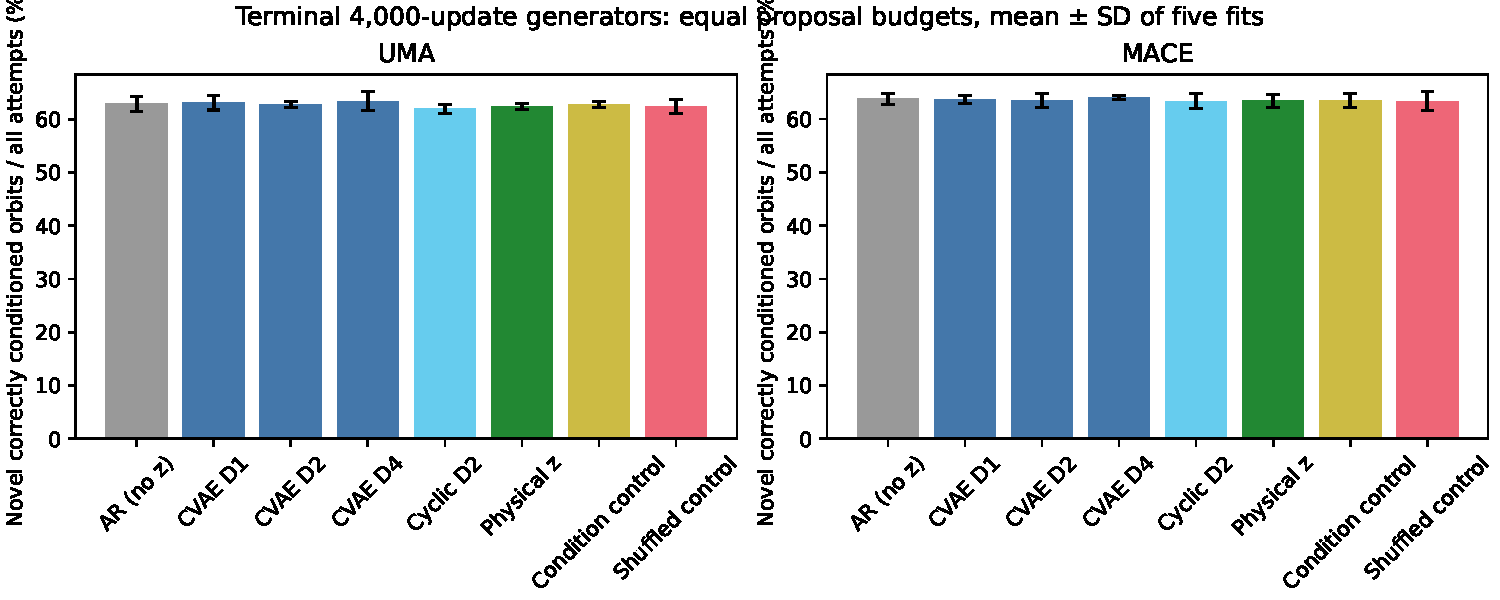
\includegraphics[width=\linewidth]{primary_oracle_yields.pdf}
\caption{Fresh first-phase development proposals, scored with both teachers.
The primary terminal checkpoints receive equal 4,000-update budgets. Error
bars describe five paired fit/proposal replicates; this pool differs from
historical assessments.}
\end{figure}

Mean terminal validation KL is 0.00291, 0.00530, and 0.01122 nats per mask
for $D=1,2,4$, respectively. None of these fits has an encoder-mean coordinate
with variance above the provisional $10^{-3}$ diagnostic threshold. This
threshold is a reporting convention, not a universal definition of a useful
latent dimension. Reconstruction can continue improving while KL becomes
small; the cyclic schedule gives a transient KL response but no primary
sampling gain.

For the $\lambda=1$ genuine latent head, mean VAL MSE on sampled posterior
latents is 1.020486. The condition-only head gives 1.020411 and a
conditions-only ridge probe gives 1.020435. These are effectively constant
predictors on the standardized target. This pooled additive ridge probe
shows no practically resolved VAL-MSE gain from $\mu$; it does not rule out
a small within-condition signal or one requiring condition-dependent slopes.
Optimizing $z$ toward the head's quartile targets changes actual generated
pair fractions only weakly. Signed paired mean energy responses over jointly
eligible scored pairs are of order $10^{-6}$\,eV/atom, and shuffled heads can
be similarly responsive. This is not a bound on individual energy changes.
A slightly moving predictor or changed occupancy is therefore
not evidence of controlled physical ordering.

\begin{figure}[htbp]
\centering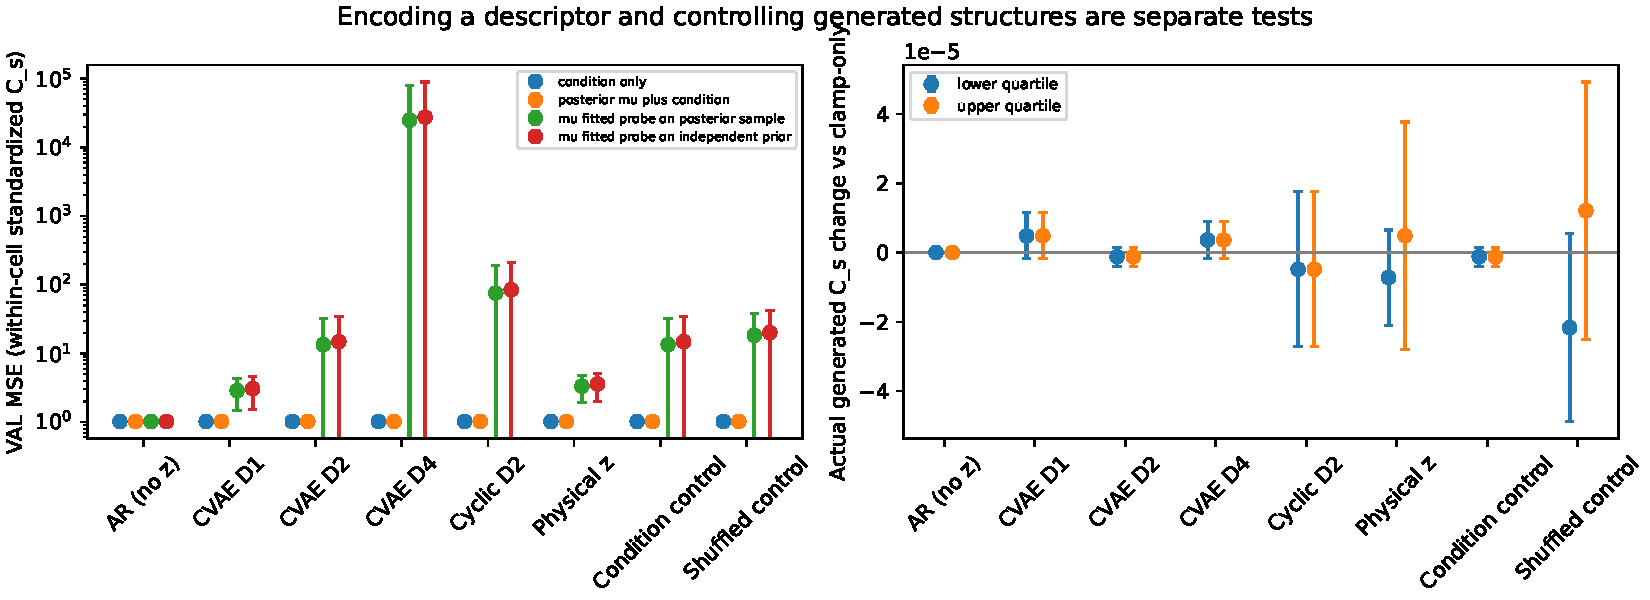
\includegraphics[width=\linewidth]{latent_physics_diagnostics.pdf}
\caption{Posterior information, held-out probes, and actual descriptor
responses to latent interventions. Prediction is tested against genuine
VAL targets; interventions are checked on generated structures rather than
only on the auxiliary head's output.}
\end{figure}
\begin{figure}[htbp]
\centering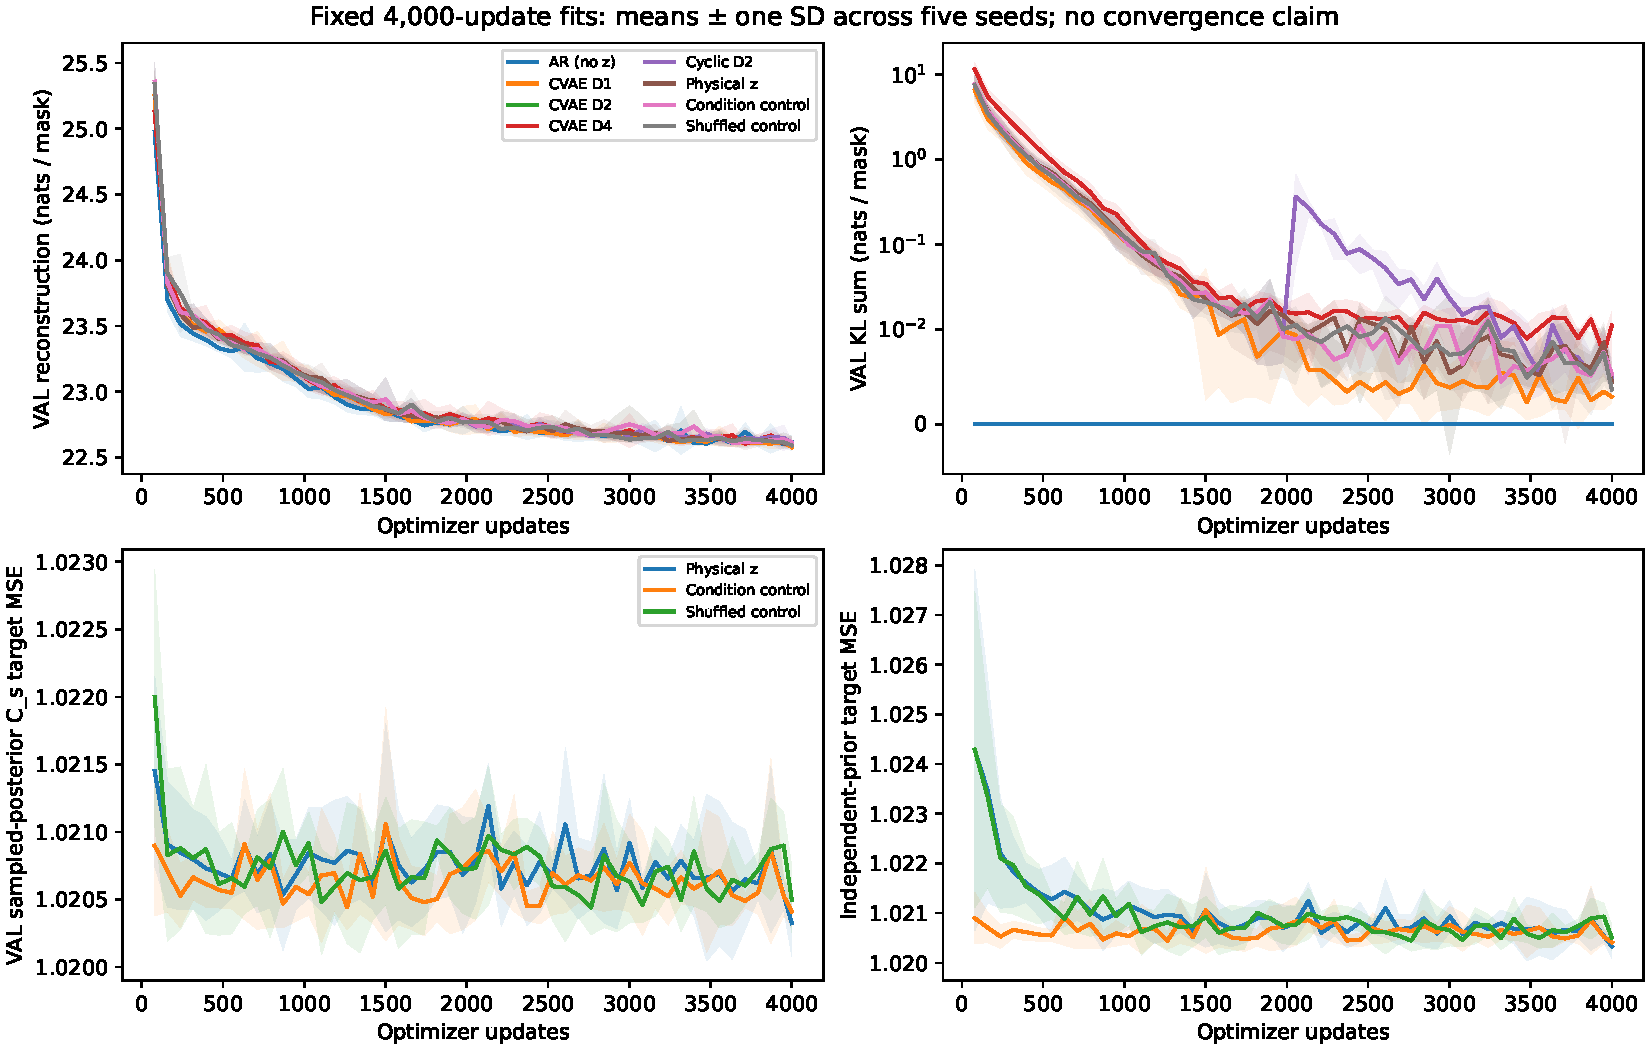
\includegraphics[width=0.97\linewidth]{optimization_curves.pdf}
\caption{Training and validation trajectories for the first phase. The
recorded 4,000-update budget is a matched comparison; slowly changing curves
do not establish optimizer convergence or physical validity.}
\end{figure}

\subsection{Does a stronger ordering loss rescue the latent vector?}
The second phase completed 30 new fits: weights 10 and 100, each crossed
with genuine, condition-only, and shuffled heads, for five seeds. Original
AR and $D=2$ references were reevaluated on the same new diagnostic streams.
The raw union contains 26,110 orbits; 25,675 were new and eligible after
excluding the shared history. Each teacher evaluated all eligible structures
afresh. This comparison has its own novelty history and should be read
within its table.

\begin{table}[htbp]
\centering\small
\caption{Primary balanced novel correct-bin yield, percent, mean $\pm$ sample SD over five fit/proposal seeds. Compare arms within this phase's fresh development history.}
\begin{tabular}{lrr}\toprule
Model & UMA & MACE\\\midrule
AR & $61.75\pm2.32$ & $63.19\pm2.01$\\
CVAE $D=2$ / condition controls & $61.04\pm3.72$ & $62.20\pm3.74$\\
Genuine head, $\lambda=10$ & $61.41\pm3.87$ & $62.36\pm3.57$\\
Shuffled target, $\lambda=10$ & $60.59\pm3.26$ & $61.60\pm2.99$\\
Genuine head, $\lambda=100$ & $61.79\pm4.02$ & $63.00\pm3.22$\\
Shuffled target, $\lambda=100$ & $62.26\pm3.59$ & $63.16\pm3.32$\\
\bottomrule\end{tabular}
\end{table}


On sampled posterior latents, the genuine head's mean VAL MSE is
$1.020409\pm0.000255$ for $\lambda=10$ and
$1.020514\pm0.000433$ for $\lambda=100$, with spread over five fits.
Mean KL rises to about 0.0312 nats/mask at $\lambda=100$, but stronger KL is
not accompanied by useful prediction or ordering control. The measured
upper-minus-lower guided change in generated pair fraction is approximately
$-10^{-6}$ and $-3.1\times10^{-5}$, respectively, even having the wrong
average sign for the requested direction.

There is one small positive sampling contrast worth preserving. On UMA,
genuine $\lambda=100$ exceeds its condition-only control by 0.746 percentage
points, with an exploratory paired 95\% interval half-width of 0.658 points.
It differs from AR by only 0.035 points and from the shuffled-target model
by $-0.469$ points. This does not identify physical information as the cause
of the gain. The ordering tests, AR comparator, and shuffled comparator are
needed to avoid that inference.

A separate 512-row TRAIN gradient audit verifies manual edge products,
target scaling, and shuffled assignments for all 45 auxiliary models from
the first two phases. Mean genuine auxiliary encoder-gradient norms increase
from approximately 0.00104 to 0.0100 to 0.1348 as $\lambda$ increases from 1
to 10 to 100; the condition-only path is exactly zero. These unweighted
diagnostic norms are not the actual weighted training update or a
convergence criterion. They establish that the target reaches the encoder
and that its strength changes; a disconnected-loss explanation is therefore
insufficient. All ten stronger condition-only controls also reproduce their
ordinary $D=2$ generator tensors and raw proposals exactly.

\subsection{Posterior-mean supervision and a more informative latent diagnosis}
The posterior-mean objective completed all 15 new fits and the 40 matched
diagnostic evaluations, including sampled-head and AR/$D=2$ references.
There were 24,586 raw unique orbits and 24,568 eligible new orbits, evaluated
by both teachers. On this fresh pool, mean-supervised yield is
$63.33\pm1.76$\% under UMA, compared with $63.47\pm0.86$\% for AR and
$63.40\pm2.05$\% for sampled-head supervision. The paired mean-minus-AR
difference is $-0.139$ percentage points, with 95\% interval half-width
1.874 points. MACE gives $64.08\pm1.85$\% for mean supervision and
$64.20\pm1.19$\% for AR. The actual guided upper-minus-lower pair-fraction
response is $(-9.65\pm23.1)\times10^{-6}$ over five fits, again having no
useful directed effect. Its auxiliary gradient reaches the encoder through
$\mu$ without a direct path through $\log\sigma^2$; shared encoder parameters,
reconstruction, and KL can still change the variance. The negative result
is not explained by a missing gradient.

An important distinction emerges from a posthoc diagnostic. The original
ridge probe standardized $\mu$ across mixed-condition data and used a common
latent slope. Large differences between conditions can obscure tiny,
condition-specific structure signals. We therefore fit an additional ridge
probe separately within each condition, scaling each latent coordinate using
TRAIN moments from that cell. The ridge strength stays at one, without
tuning; VAL targets remain held out. Balanced VAL MSE across nine cells is
$0.1009\pm0.0963$ for ordinary $D=2$, $0.0991\pm0.0644$ for sampled-head
supervision, and $0.0759\pm0.0823$ for mean supervision, versus 1.0212 for
the TRAIN-zero reference and approximately 1.025 for shuffled-target probes.
Thus the deterministic mean retains a recoverable ordering fingerprint.

This fingerprint is not necessarily learned. In the fixed 24-Li, MIDDLE-bin
cell, five random-initialized graph encoders give probe MSE
$0.00671\pm0.00591$, compared with $0.0809\pm0.0567$ for trained $D=2$.
Nonlinear message passing and pooling already encode pair correlations
through the supplied physical graph. These random-feature controls prevent
interpreting a colored latent scatter as evidence that training discovered a
useful physical coordinate.

\begin{figure}[htbp]
\centering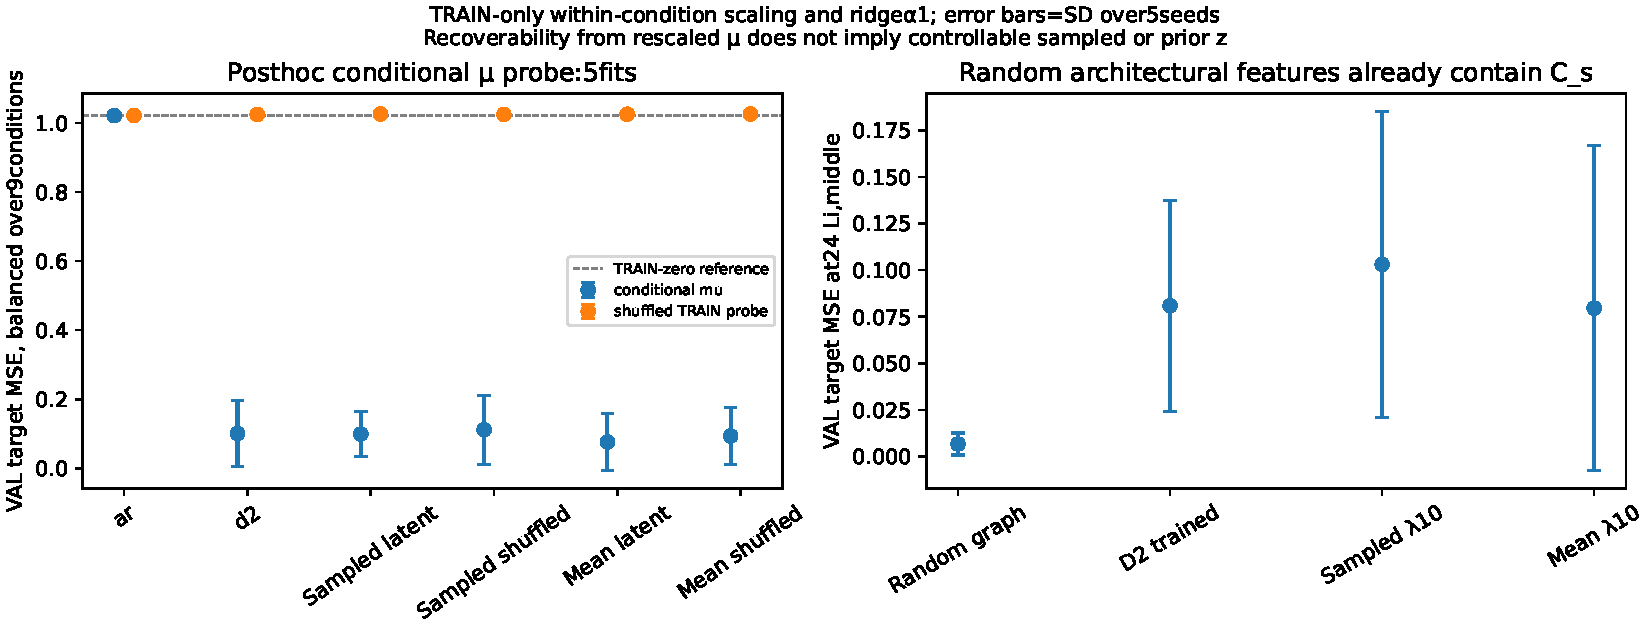
\includegraphics[width=\linewidth]{conditional_information_comparison.pdf}
\caption{Posthoc probes with TRAIN-only within-condition scaling. Left:
balanced held-out MSE over the nine cells, with five-fit SD. Right:
fixed-condition random-encoder and trained-encoder comparisons. The
nearest-shell vacancy-pair fraction, called $C_s$ in the plots, is
$C_{\rm vv}$ in the equations. These probes read deterministic means.}
\end{figure}

The scale matters. In the predeclared first-fit illustration with 986 VAL
records at fixed count and energy bin, SD$(\mu_1)$ is approximately
$1.29\times10^{-6}$ for ordinary $D=2$, $1.63\times10^{-7}$ for sampled-head
supervision, and $2.45\times10^{-8}$ for mean supervision. Posterior standard
deviations are about 0.94--0.96 and the prior standard deviation is one.
A rescaled scatter can reveal ordering in $\mu$, while adding unit-scale
Gaussian noise almost completely hides that ordering from sampled $z$.
For illustration, two equal-unit-variance Gaussians whose means differ by
$10^{-6}$ have KL $\tfrac12(10^{-6})^2=5\times10^{-13}$ nats. This example
explains the scale; it is not a substitute for the measured posteriors.

\begin{figure}[p]
\centering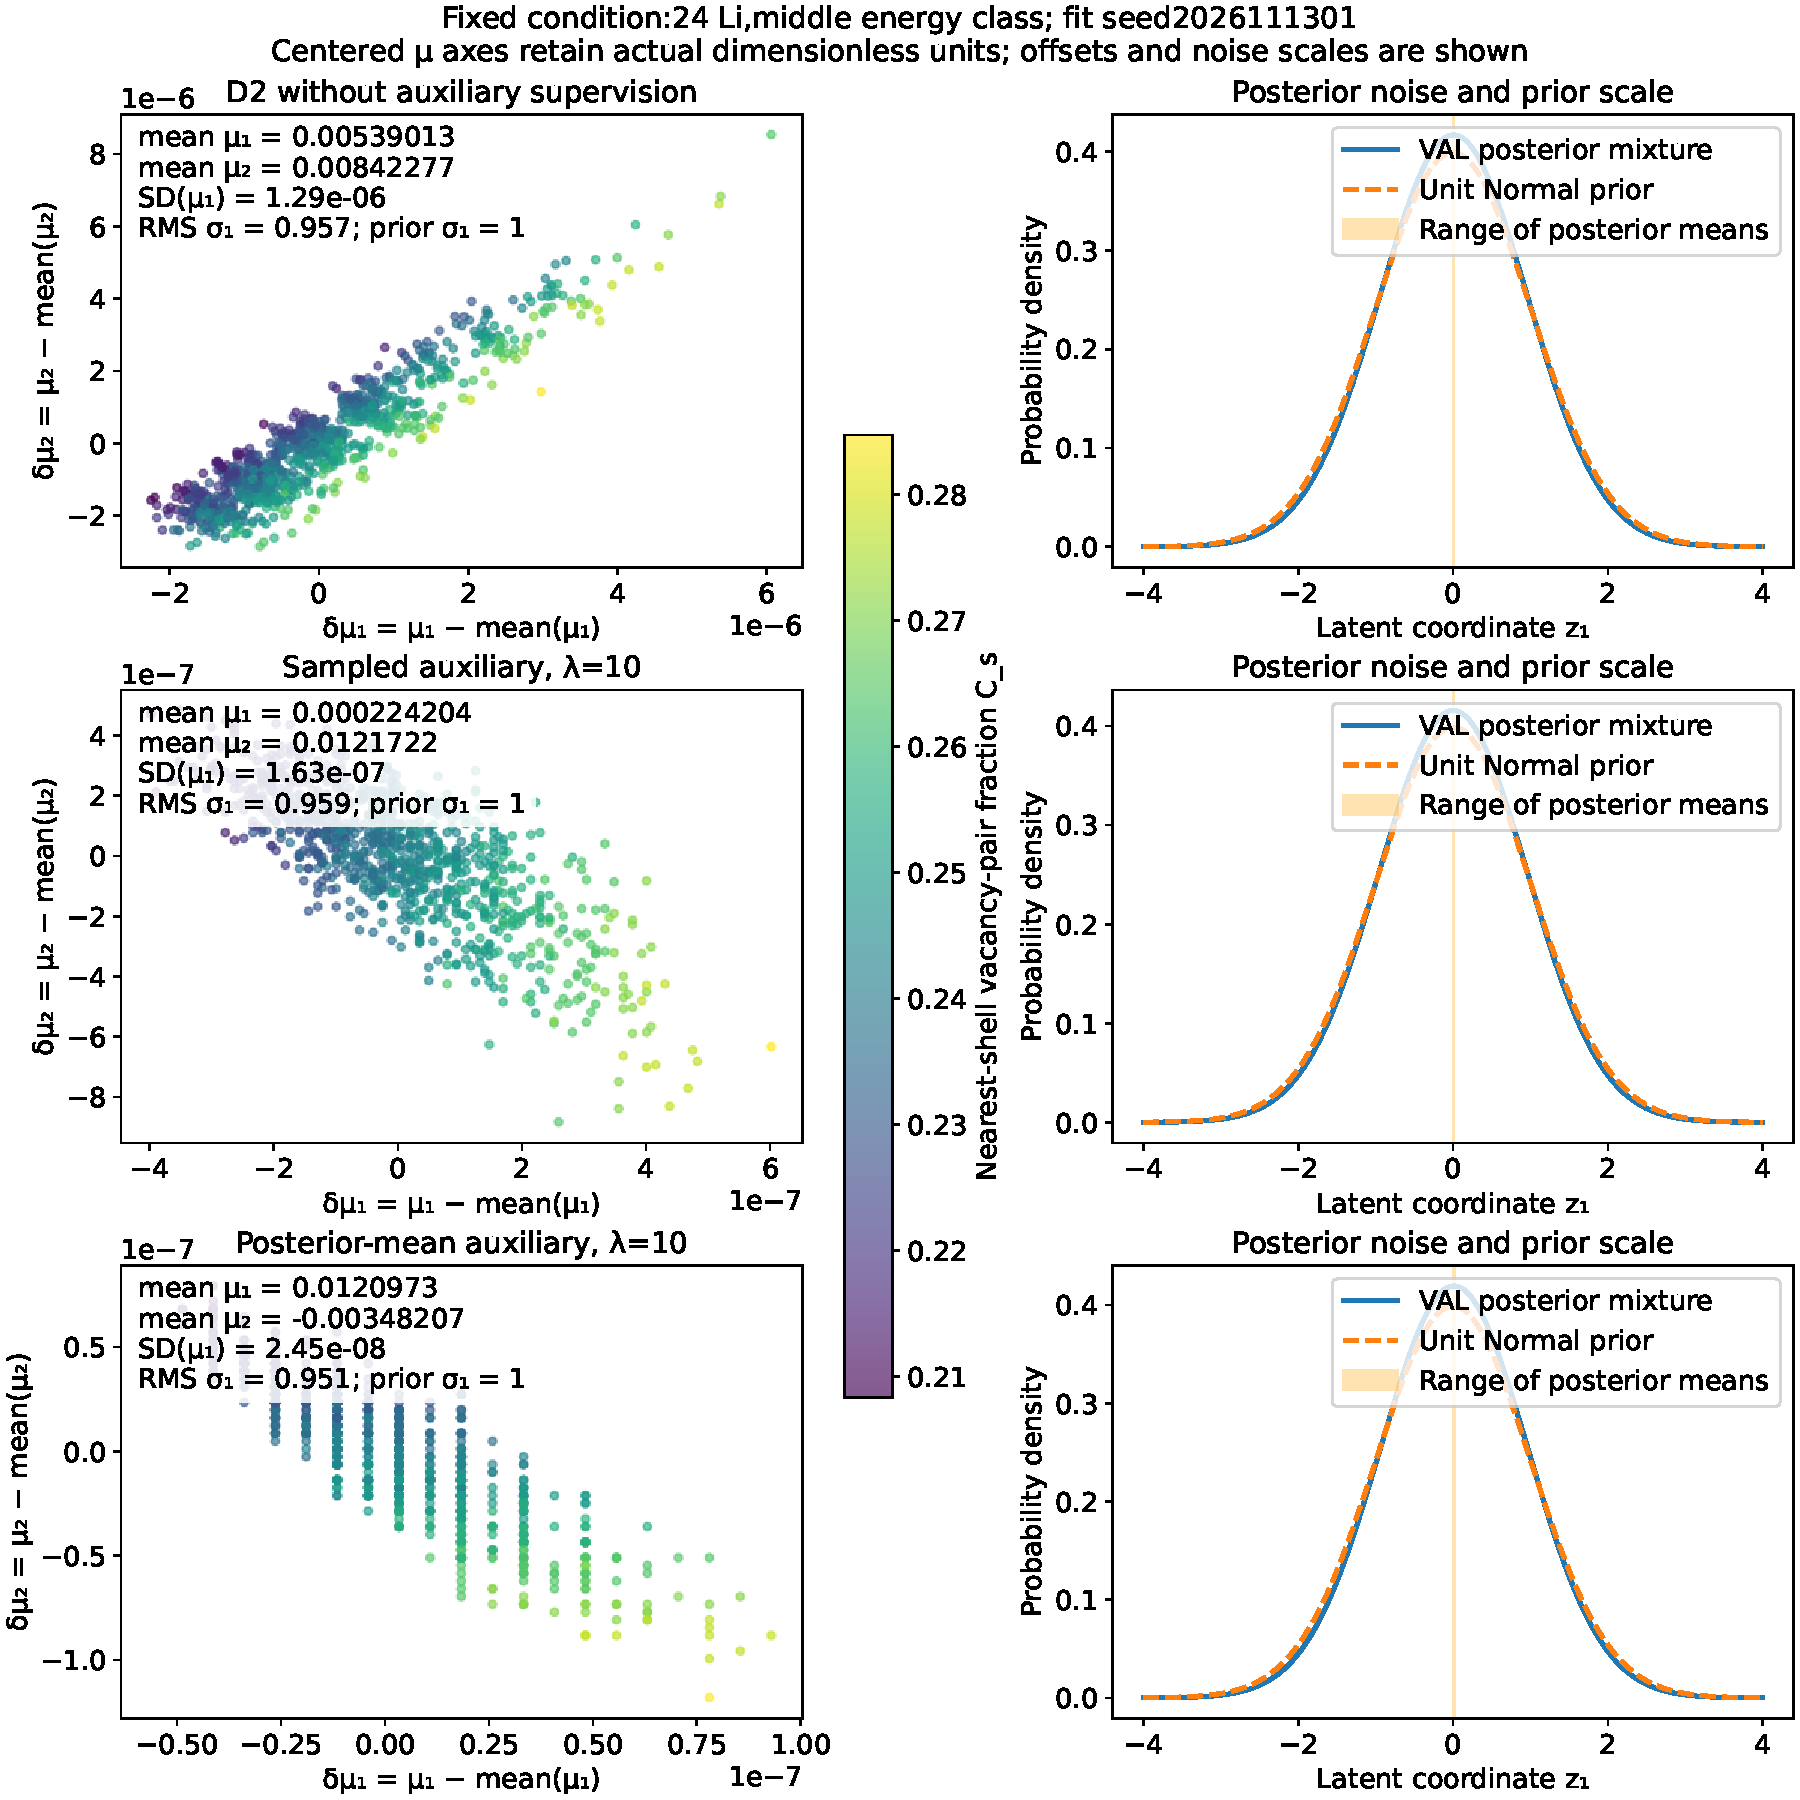
\includegraphics[width=\linewidth,height=0.85\textheight,keepaspectratio]{fixed_condition_latent_centered.pdf}
\caption{One predeclared fit and condition: $n=24$, MIDDLE, seed 2026111301.
Centered mean coordinates reveal the tiny structure-dependent variation;
the accompanying posterior-mixture panels show it relative to sampling
noise. Encoder outputs here are CPU FP32 reevaluations; moment statistics
use float64. The primary generation retains its GPU protocol. This illustration is not a selected
best fit, and its colored means do not establish prior-generation control.}
\end{figure}

We can quantify this distinction without estimating mutual information from
a scatter. Let $q_i$ be the diagonal Gaussian encoder posterior of VAL mask
$i$ in this fixed cell, and $\bar q=N^{-1}\sum_jq_j$. Take the uniform
empirical distribution over the $N=986$ VAL records. Then
\begin{equation}
I_{\rm VAL}(X;Z\mid c)=\frac1N\sum_i\KL(q_i\|\bar q)
\;\leq\;\frac1{N^2}\sum_{i,j}\KL(q_i\|q_j).
\end{equation}
The inequality follows from convexity of $-\log$:
$-\log[N^{-1}\sum_jq_j(z)]\leq N^{-1}\sum_j[-\log q_j(z)]$.
Integrating under each $q_i$ and averaging gives the right-hand side.
Pairwise Gaussian KL is analytic. A cancellation-resistant
float64 calculation, checked with an independent Gaussian implementation,
80-digit spot calculations, and a Taylor upper envelope, gives:

\begin{table}[htbp]
\centering\small
\caption{Information diagnostics for the fixed empirical VAL cell and first
fit only. The pairwise quantity is a computed upper bound, reported by order
of magnitude rather than as interval-certified last digits.}
\begin{tabular}{lrr}\toprule
Encoder & Mean KL to prior (nats) & Pairwise information bound (nats)\\\midrule
Ordinary $D=2$ & $4.06\times10^{-3}$ & $\sim7.1\times10^{-12}$\\
Sampled-head $\lambda=10$ & $3.48\times10^{-3}$ & $\sim4.2\times10^{-13}$\\
Mean-head $\lambda=10$ & $6.56\times10^{-3}$ & $\sim4.8\times10^{-15}$\\\bottomrule
\end{tabular}
\end{table}

Most KL to the prior in this illustration describes a common mismatch of
the conditional posterior mixture, rather than information distinguishing
the masks. This is a statement about the empirical encoder joint
$(X,Z)$ in one cell. It does not prove that the decoder ignores prior $z$;
the prior interventions and generated-property measurements test that
separate question. Together, they explain how informative deterministic
means can coexist with ineffective sampled-latent physical control.

The conditional probes and numerical checks introduce no new training or
oracle calls. An initial float32 moment annotation at this extremely small
scale was corrected using float64; original plots are preserved with the
precision-correction receipt. The figures here use the corrected values.




\section{Adaptive energy labels and two acquisition rounds}
At a fixed composition, the meaning of ``low energy'' can be updated after
new structures are evaluated. We compare three rules fitted only to TRAIN:
\begin{align}
\text{fixed:}\quad &(a,b)=(a_0,b_0),\\
\text{adaptive quantiles:}\quad &(a,b)=(Q_{0.2},Q_{0.8}),\\
\text{observed range:}\quad &(a,b)=(E_{\min}+0.2R,E_{\min}+0.8R),\quad
R=E_{\max}-E_{\min}.
\end{align}
Energies here are eV per atom within one composition. The first rule preserves
the original semantics. Quantiles keep empirical class populations roughly
balanced but depend on which samples were acquired; finding a new minimum
does not necessarily move the 20th percentile much. The range rule responds
to observed extrema, but a single outlier can shift it substantially and
leave a bin with little support. Neither rule knows the global endpoints or
turns conditional sampling into gradient descent. Ties, class support,
observed endpoints, and actual boundary movement are retained in the output.

Three paired seeds and both AR and $D=2$ CVAE are followed through two rounds.
Every acquisition requests all nine count--bin cells with 512 attempts and
at most 256 first eligible unique queries per cell. Candidates are selected
without seeing energy; every successfully evaluated selected candidate is
added to TRAIN and labeled by its \emph{measured}, rather than requested,
energy. The three relabeling rules share exactly the same first acquired
batch for a given model and seed. Their first-round contrast therefore
isolates the label-definition policy and its induced class weighting on the
same enriched data; second-round candidate sets
may diverge and the comparison becomes one of adaptive policies.

Each update is a 2,000-step model-weight warm start with a new optimizer and
declared random stream. Every updated lineage has an equal-update no-new-data
continuation. In round two, that control begins at the same first-round
checkpoint and uses its previous data and schema. Its paired contrast
measures the combined acquisition-and-rebinning policy, not a label-only
effect. Added rows also change minibatches and class weights. Fresh
assessments use 128 attempts per cell, fixed teacher-specific evaluation bins,
and the same novelty history for all arms. Moving-bin success is reported
separately. UMA's adaptive training bins must not be applied to MACE's
absolute energies. Uniform fixed-count sampling and mutation from a frozen,
unprotected original TRAIN seed bank retain their own equal proposal/query
budgets.

The acquisition query cap makes Eq.~\ref{eq:yield} at most 0.5 in those
acquisition tables, even if all queries are successful. Fresh assessments
allow one query per attempt. These two table types must not be compared as
though they had the same attainable yield. Endpoint discovery is measured
within composition; changing lithium count also changes chemistry and the
number of atoms, so an average absolute energy across counts is not a
formation energy or a physical ranking.

\subsection{A first-round gain that does not persist under the same metric}
All four core acquisition/assessment phases pass the original strict raw
verifier. Each teacher evaluates 25,215 first-round acquisition geometries,
23,504 first-round assessment geometries, 40,301 second-round acquisition
geometries, and 27,725 second-round assessment geometries: 233,490
geometry--teacher evaluations in total. The first round adds exactly 2,304
new TRAIN rows per model/seed, shared across its three label policies.

\begin{table}[htbp]
\centering\small
\caption{Change in balanced H0 fixed-bin yield versus an equal-update no-new-data continuation, in percentage points, mean $\pm$ sample SD over three paired fit/proposal seeds. Round 2 uses the same first-round lineage as its control. The rounds have separate assessment histories.}
\begin{tabular}{lrrrr}\toprule
Model / rule & UMA r1 & UMA r2 & MACE r1 & MACE r2\\\midrule
AR / fixed & $-1.33\pm1.61$ & $+1.39\pm0.53$ & $-1.50\pm0.85$ & $+1.27\pm0.35$\\
AR / adaptive & $-0.35\pm1.51$ & $+0.61\pm0.60$ & $+0.03\pm2.23$ & $+0.14\pm0.90$\\
AR / range & $+6.57\pm2.36$ & $-5.41\pm1.48$ & $+6.13\pm1.35$ & $-6.31\pm1.65$\\
CVAE $D=2$ / fixed & $-0.90\pm0.88$ & $-0.17\pm0.68$ & $-0.69\pm1.00$ & $-0.55\pm0.56$\\
CVAE $D=2$ / adaptive & $+0.17\pm1.61$ & $+0.43\pm0.63$ & $+0.12\pm1.66$ & $+0.26\pm0.77$\\
CVAE $D=2$ / range & $+6.08\pm1.97$ & $-6.28\pm1.76$ & $+6.16\pm1.25$ & $-6.22\pm1.48$\\
\bottomrule\end{tabular}
\end{table}

\begin{table}[htbp]
\centering\small
\caption{Declared broad three-bin sampling baselines: balanced H0 yield in percent, mean $\pm$ three-seed SD. Mutation uses its frozen original-TRAIN seed bank. These numbers do not replace earlier LOW-only or differently seeded mutation studies.}
\begin{tabular}{llrr}\toprule
Round & Teacher & Uniform & Mutation\\\midrule
1 & UMA & $34.06\pm1.94$ & $58.36\pm0.53$\\
1 & MACE & $33.19\pm1.37$ & $57.18\pm0.41$\\
2 & UMA & $33.88\pm0.59$ & $58.16\pm1.53$\\
2 & MACE & $33.68\pm1.51$ & $56.63\pm1.18$\\
\bottomrule\end{tabular}
\end{table}


Observed-range labels give a clear first-round balanced-yield gain relative
to the declared no-new-data continuation. The same-data contrast is also
positive: range minus fixed gives $+7.90\pm0.83$ percentage points for AR
and $+6.97\pm2.74$ for $D=2$ under UMA; MACE gives $+7.64\pm0.76$ and
$+6.86\pm2.25$. These are three-fit sample SDs. This isolates the effect of
label definitions and induced class weighting on the same augmented rows,
rather than proving that acquisition itself was necessary.

The improvement is not uniform across requested classes. For AR, the
range-minus-fixed change is only $+0.35$ points for fixed-H0 LOW yield but
$+29.77$ points for HIGH yield. A balanced three-class gain should therefore
not be described as an equivalent gain in low-energy discovery. The
declared uniform and mutation baselines remain below the neural models in
this broad three-bin assessment. Different seed-selection or LOW-only
mutation studies have a different target and cannot be substituted here.

\begin{figure}[htbp]
\centering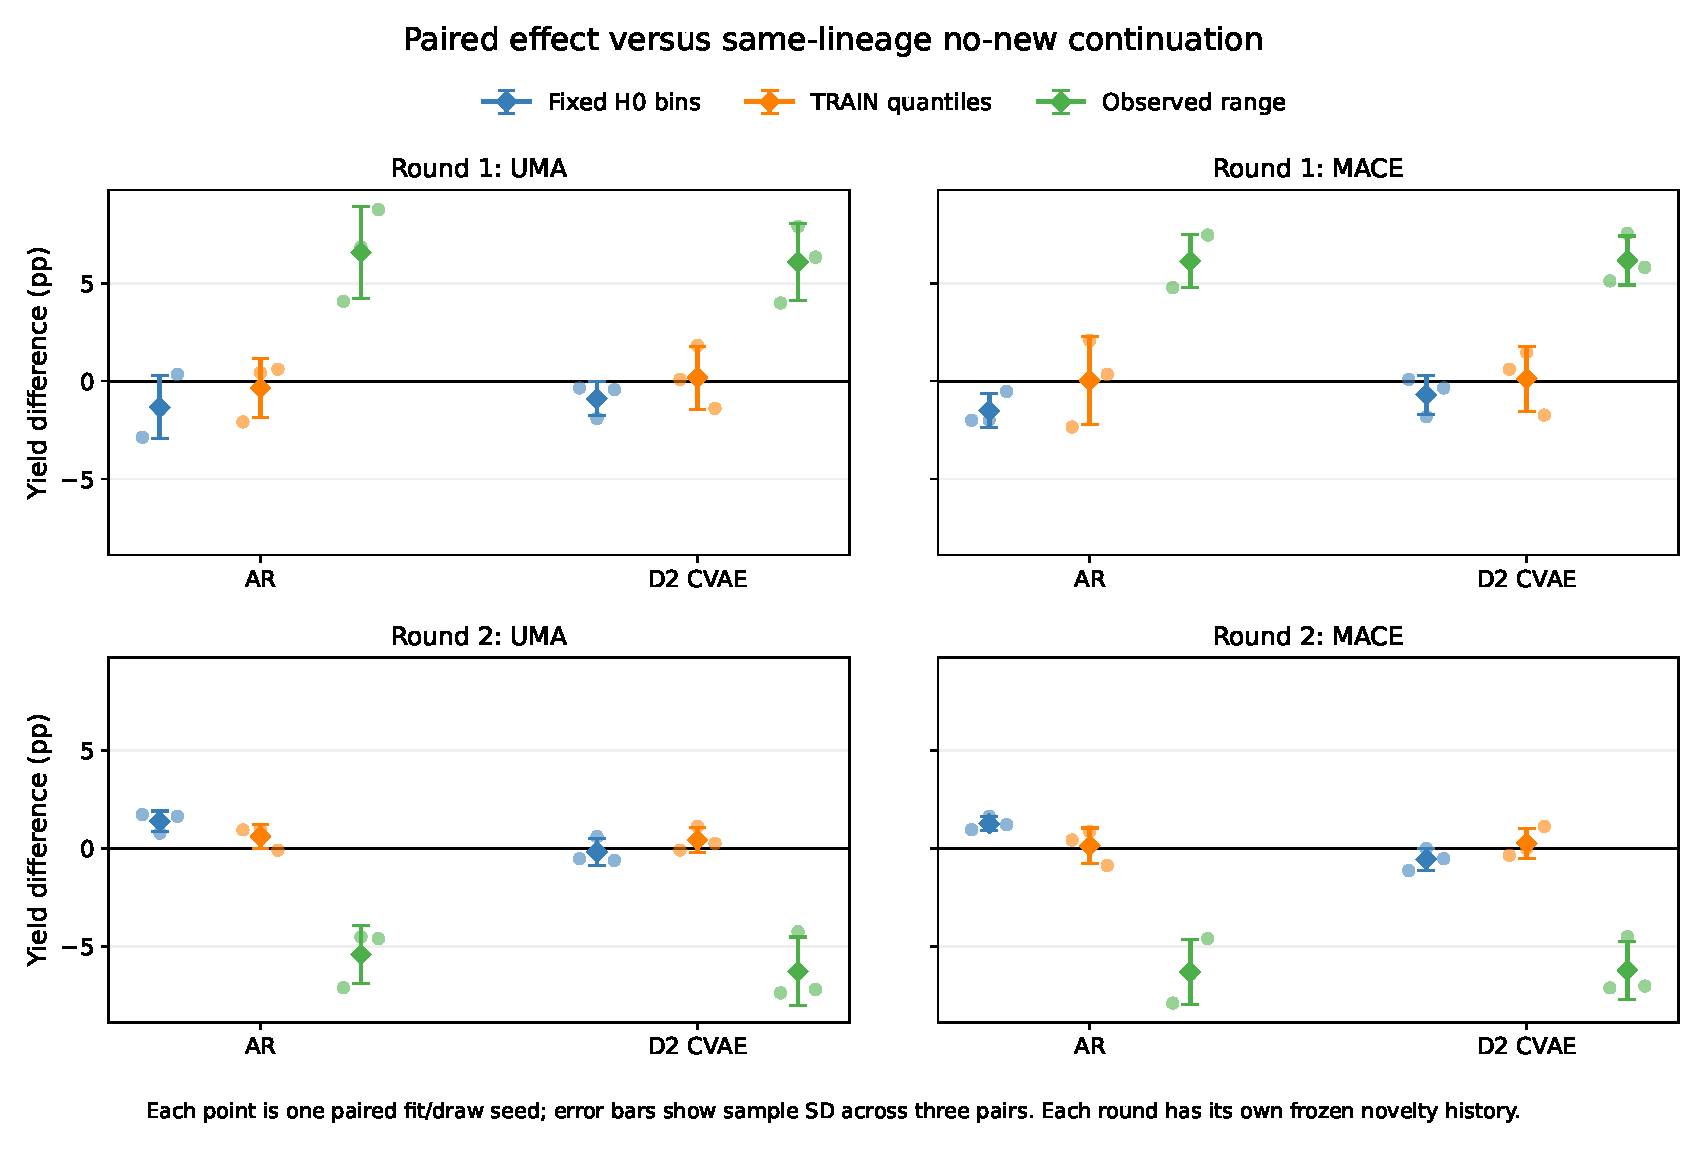
\includegraphics[width=\linewidth]{iteration_paired_gains.pdf}
\caption{Paired effects relative to the appropriate equal-update
continuation. Round 1 compares with H0 continuation; round 2 compares with
the same first-round lineage continued without a new batch. Individual
replicates and three-fit SD are shown. Fixed-H0 evaluation bins remain
constant; the novelty history is separately frozen for each round.}
\end{figure}

In round two, the range policy loses $5.41\pm1.48$ points for AR and
$6.28\pm1.76$ for $D=2$ relative to its same-lineage no-new-data control
under UMA. MACE gives corresponding losses of $6.31\pm1.65$ and
$6.22\pm1.48$ points. Absolute UMA range yields are 70.28\% and 68.66\%,
compared with the fresh uniform baseline 33.88\% and mutation 58.16\%.
Thus the neural sampler remains useful against these declared baselines,
while adding another range-policy batch does not sustain the first-round
improvement in the fixed-reference statistic.

\subsection{Novelty, condition fidelity, and the moving target}
Existing-result diagnostics separate novelty $N$ from conditional accuracy
$A$ among scored new orbits. Within each cell, $Y=NA$. The exact symmetric
rate decomposition is
\begin{equation}
\Delta Y=\tfrac12(A_1+A_0)\Delta N+
          \tfrac12(N_1+N_0)\Delta A.
\end{equation}
Balanced cell averages therefore retain an exact arithmetic decomposition;
it does not identify the causal training mechanism. For UMA range AR, the
round-two change is approximately $-1.06$ percentage points from the novelty
term and $-4.36$ from conditional accuracy. For $D=2$ the terms are
$-1.97$ and $-4.31$ points. Novelty remains 98.41\%/97.34\%, versus
99.51\%/99.33\% in the respective continuations. The dominant measured
change is condition fidelity, rather than wholesale repetition of known
patterns. Some LOW cells lose roughly 14 points despite almost complete
novelty.

There is an important target-alignment explanation to examine. For a
range-defined lower cutoff $a=0.8E_{\min}+0.2E_{\max}$,
$\Delta a=0.8\Delta E_{\min}+0.2\Delta E_{\max}$. The range acquisition
mostly extends the \emph{upper} energy endpoint, while its lower endpoint
changes much less. Raising $E_{\max}$ also raises the definition of LOW.
The generator can consequently match a broader, higher-energy LOW class
while losing hits under the original fixed-H0 LOW threshold. Moving-bin
fidelity and observed endpoint growth are therefore reported separately;
the fixed-yield loss alone does not establish failure to extend upper-energy
coverage. Nor does extending an observed range prove global coverage or
convergence.

\begin{figure}[htbp]
\centering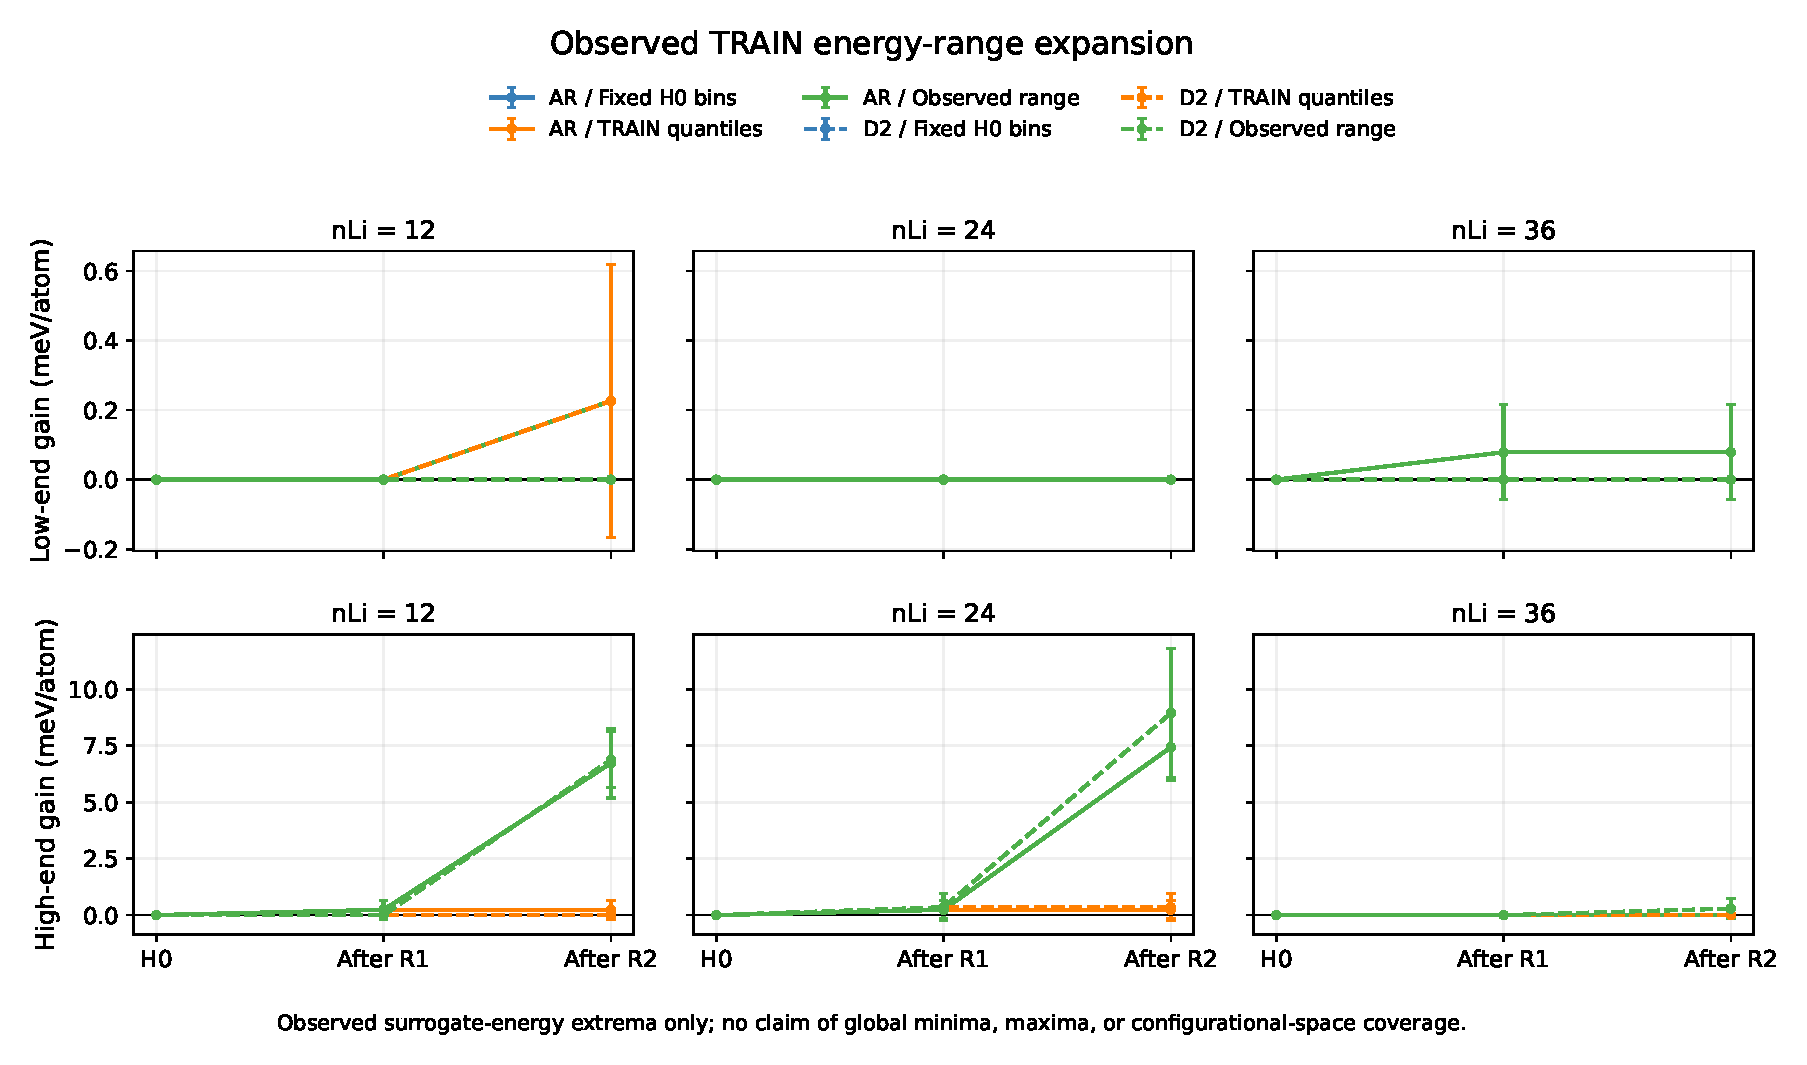
\includegraphics[width=\linewidth]{observed_training_extrema_growth.pdf}
\caption{Observed TRAIN endpoint extension relative to H0, within each
composition. Positive lower-endpoint growth means a lower observed minimum;
positive upper-endpoint growth means a higher maximum. These nested TRAIN
data can be compared longitudinally, unlike assessment yields with changing
novelty histories. Error bars are three-seed SD, not bounds on global extrema.}
\end{figure}

Range labels also concentrate the loss on rare examples. One first-round
36-Li HIGH class has only three TRAIN structures among roughly 14,000.
Class balancing changes per-row loss weights, not the uniformly shuffled
minibatch order. If those three examples carry one third of the within-count
loss mass, Cauchy's inequality gives $\sum_i p_i^2\geq1/27$ for normalized
weights $p_i$, hence weight ESS $1/\sum_i p_i^2\leq27$. This is concentration
of objective weight, not 27 independent physical observations. The first
round's positive result means sparsity alone cannot be cited as the cause
of the second-round loss. Actual class support, edge shifts, endpoint motion,
and weight ESS are all retained for each lineage.

\subsection{Does the first range-label gain require new structures?}
A post-hoc control separates two changes that occurred together in the first
round: adding newly evaluated structures and redefining their energy classes.
This follow-up was prompted by the first-round result; it is a mechanistic
test, not a new blind confirmation. Its plan and paired fit/proposal seeds were
frozen before the follow-up fits.

For each architecture and each of the three seeds, the comparison starts from
the same original 4,000-update checkpoint and allocates another 2,000 updates.
The original H0 data and first-round augmented data are each evaluated with
fixed bins and with identical range-bin edges. Existing equal-update
checkpoints supply the H0/fixed and augmented-data comparisons. We additionally
fit H0 with range edges estimated from H0 TRAIN alone, which tests relabeling
without any acquired labels. Some H0 and augmented-data range edges differ,
so six more H0 fits use each lineage's exact first-round range edges. These
remove edge location as a difference when testing the effect of added rows.
There are twelve new fits in total; all requested classes have actual H0
TRAIN support.

All compared checkpoints generate fresh proposals under one common history,
with 128 attempts for each count/request cell and common proposal streams.
Their energies are evaluated under the original, teacher-specific H0
assessment bins. None of these assessment labels enter training. The
comparison therefore asks whether new rows help under the same physical
energy intervals, rather than allowing the assessment target to move.

\begin{table}[htbp]
\centering\small
\caption{Posthoc conditioning/data controls: balanced H0 fixed-bin yield change, percentage points, mean $\pm$ sample SD over three paired fits. Relabeling also changes class-balanced loss weights. The matched-range comparison holds the physical edges identical; adding rows can still change minibatches and row weights.}
\begin{tabular}{lrr}\toprule
Model / contrast & UMA & MACE\\\midrule
AR / H0 range versus fixed & $+6.48\pm1.01$ & $+6.11\pm0.98$\\
AR / New rows / fixed edges & $-1.56\pm0.88$ & $-1.10\pm1.33$\\
AR / New rows / matched range edges & $-1.36\pm0.39$ & $-2.05\pm0.84$\\
CVAE $D=2$ / H0 range versus fixed & $+7.06\pm1.09$ & $+6.80\pm0.91$\\
CVAE $D=2$ / New rows / fixed edges & $+0.41\pm0.78$ & $+0.09\pm0.46$\\
CVAE $D=2$ / New rows / matched range edges & $+1.85\pm1.33$ & $+2.00\pm1.39$\\
\bottomrule\end{tabular}
\end{table}


Relabeling H0 alone recovers a large gain: $+6.48\pm1.01$ percentage points for
AR and $+7.06\pm1.09$ for $D=2$ under UMA. MACE gives
$+6.11\pm0.98$ and $+6.80\pm0.91$ points. The corresponding effect of adding
rows at identical first-round range edges is smaller and depends on the
architecture: $-1.36\pm0.39$ points for AR and $+1.85\pm1.33$ for $D=2$
under UMA, with MACE changes of $-2.05\pm0.84$ and $+2.00\pm1.39$.
Under the original fixed bins, adding rows changes UMA yield by
$-1.56\pm0.88$ for AR and $+0.41\pm0.78$ for $D=2$.
These are sample SDs over three paired fit/proposal replicates.

The large first-round gain can thus be obtained without acquiring new
structures. This supports a useful role for the definition of the conditioning
classes and the associated loss weighting. It does not establish that
acquisition is useless: added rows have a small positive effect for $D=2$
under matched range edges, and the acquisition pools extend the observed
upper-energy range. Nor does the control isolate why relabeling helps.
Relabeling changes class membership and the weights assigned by the
class-balanced loss; adding rows also changes minibatches and class weights.
The effects measured here belong to that declared training procedure.

\begin{figure}[htbp]
\centering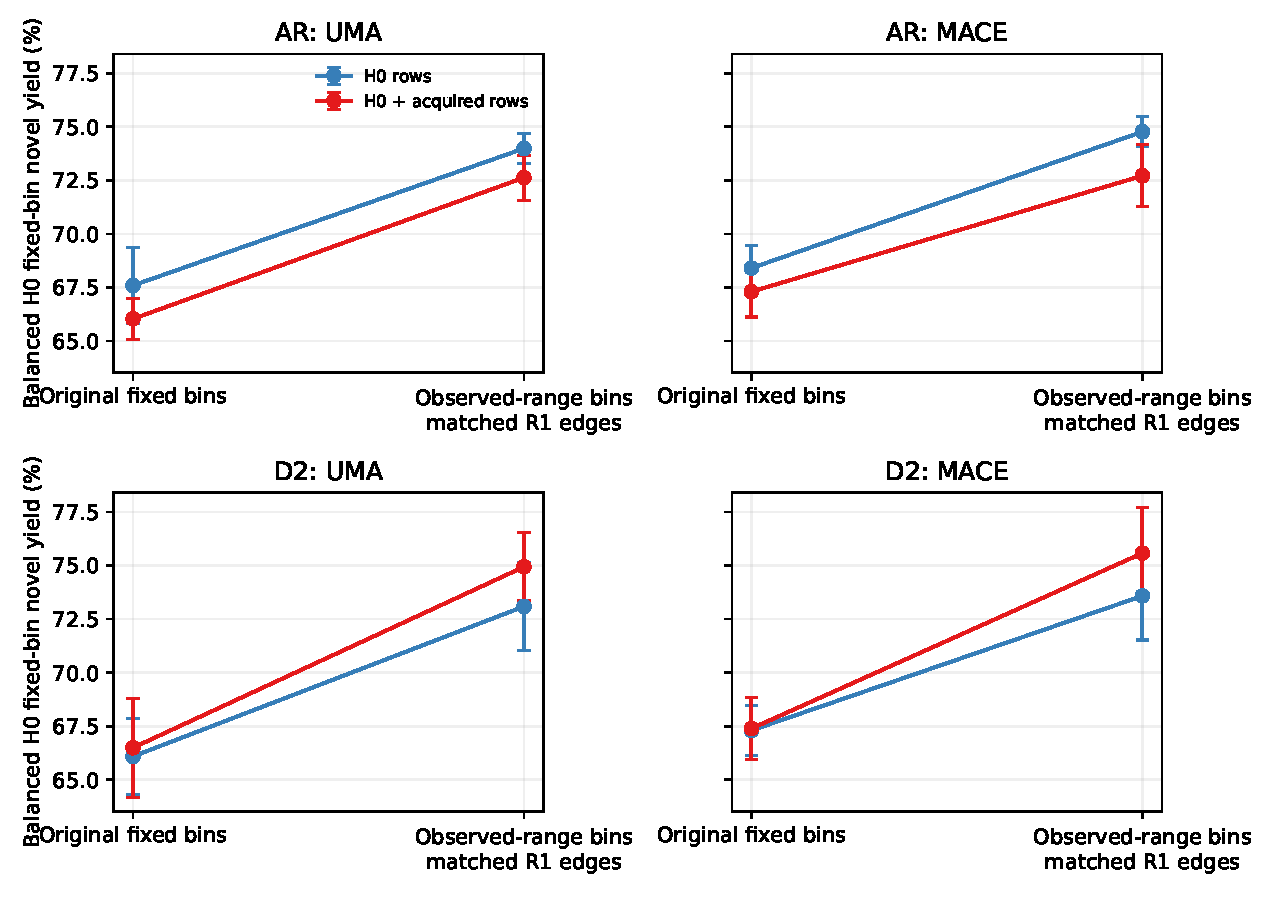
\includegraphics[width=\linewidth]{causal_factorial.pdf}
\caption{Post-hoc data-by-conditioning control on fresh common proposals.
The two data choices use identical physical condition edges at each plotted
position. The separate pure-H0 range fit, whose edges need no acquired labels,
is included in the control table. Error bars show three-pair sample SD.
The result concerns fixed-H0 conditional yield, not DFT accuracy or a
global energy minimum.}
\end{figure}

The follow-up completes in 18.04 minutes and uses 34,686 geometry--teacher
evaluations, with all raw-score checks passing. Its raw proposal identities
are reserved before the subsequent search pilot, preserving the assessment
boundary.

\subsection{A bounded test of explicit endpoint search}
Updating energy labels does not directly follow an energy gradient. We
therefore run a separate discrete search pilot to test the value of feedback
from an actual MLIP evaluation. It begins only after the core experiment is
complete and after all causal-control proposal identities have been reserved.

At each of the three lithium counts, LOW and HIGH searches begin from 16
unprotected H0 TRAIN masks per seed. Greedy and energy-blind walks share those
starts. At each of four steps, each trajectory proposes eight edits, each
exchanging one occupied and one vacant Li site. This is one swap in occupancy
space, not a physical diffusion trajectory. The greedy walk chooses the
lowest- or highest-energy eligible neighbor according to UMA; ties use a
declared canonical-mask order. The blind walk's chosen neighbor and its
eligibility-only fallback are written before any new energy is evaluated.
Both walks query the full eligible candidate union. Their first-step raw
proposals and query unions are checked to be exactly identical.

A uniform fixed-count sampler receives the same attempt/query caps, without
a claim of identical edit semantics. Each arm has at most 128 attempts and
new queries per count/direction/step, or 512 over four steps. Known,
protected, and repeated orbits remain excluded without top-ups. Actual
selected query counts are retained, and shared geometry--teacher evaluations
are physically performed only once.

\begin{table}[htbp]
\centering\small
\caption{Best observed UMA energy gain relative to the same starting-pool
best, in meV/atom, mean $\pm$ sample SD over three paired seeds. Positive
LOW gain means lower energy; positive HIGH gain means higher energy.
The reference is the best of the common 16 starts, not the minimum or
maximum of the entire H0 dataset.}
\begin{tabular}{llrrr}\toprule
Li count & Direction & Greedy & Blind walk & Uniform\\\midrule
12 & LOW  & $2.17\pm0.67$ & $1.38\pm0.97$ & $1.33\pm0.89$\\
24 & LOW  & $2.06\pm1.02$ & $1.05\pm0.65$ & $1.20\pm1.63$\\
36 & LOW  & $2.82\pm0.65$ & $1.21\pm0.29$ & $1.19\pm0.24$\\
12 & HIGH & $8.26\pm3.38$ & $3.70\pm0.14$ & $2.04\pm2.15$\\
24 & HIGH & $5.29\pm2.87$ & $4.61\pm3.34$ & $1.75\pm2.42$\\
36 & HIGH & $5.45\pm2.25$ & $1.93\pm1.31$ & $1.31\pm1.72$\\
\bottomrule\end{tabular}
\end{table}

Within this bounded budget, energy feedback improves the mean observed LOW
endpoint relative to both declared controls at all three counts. MACE audits
the same queried structures independently and shows the same qualitative
LOW advantage: greedy gains are 2.33, 2.16, and 2.46 meV/atom at counts
12, 24, and 36. MACE does not choose the next states. The HIGH advantage is
less uniform across counts and replicates, particularly at count 24.
These small paired experiments do not establish a universal ordering of
the methods.

\begin{figure}[htbp]
\centering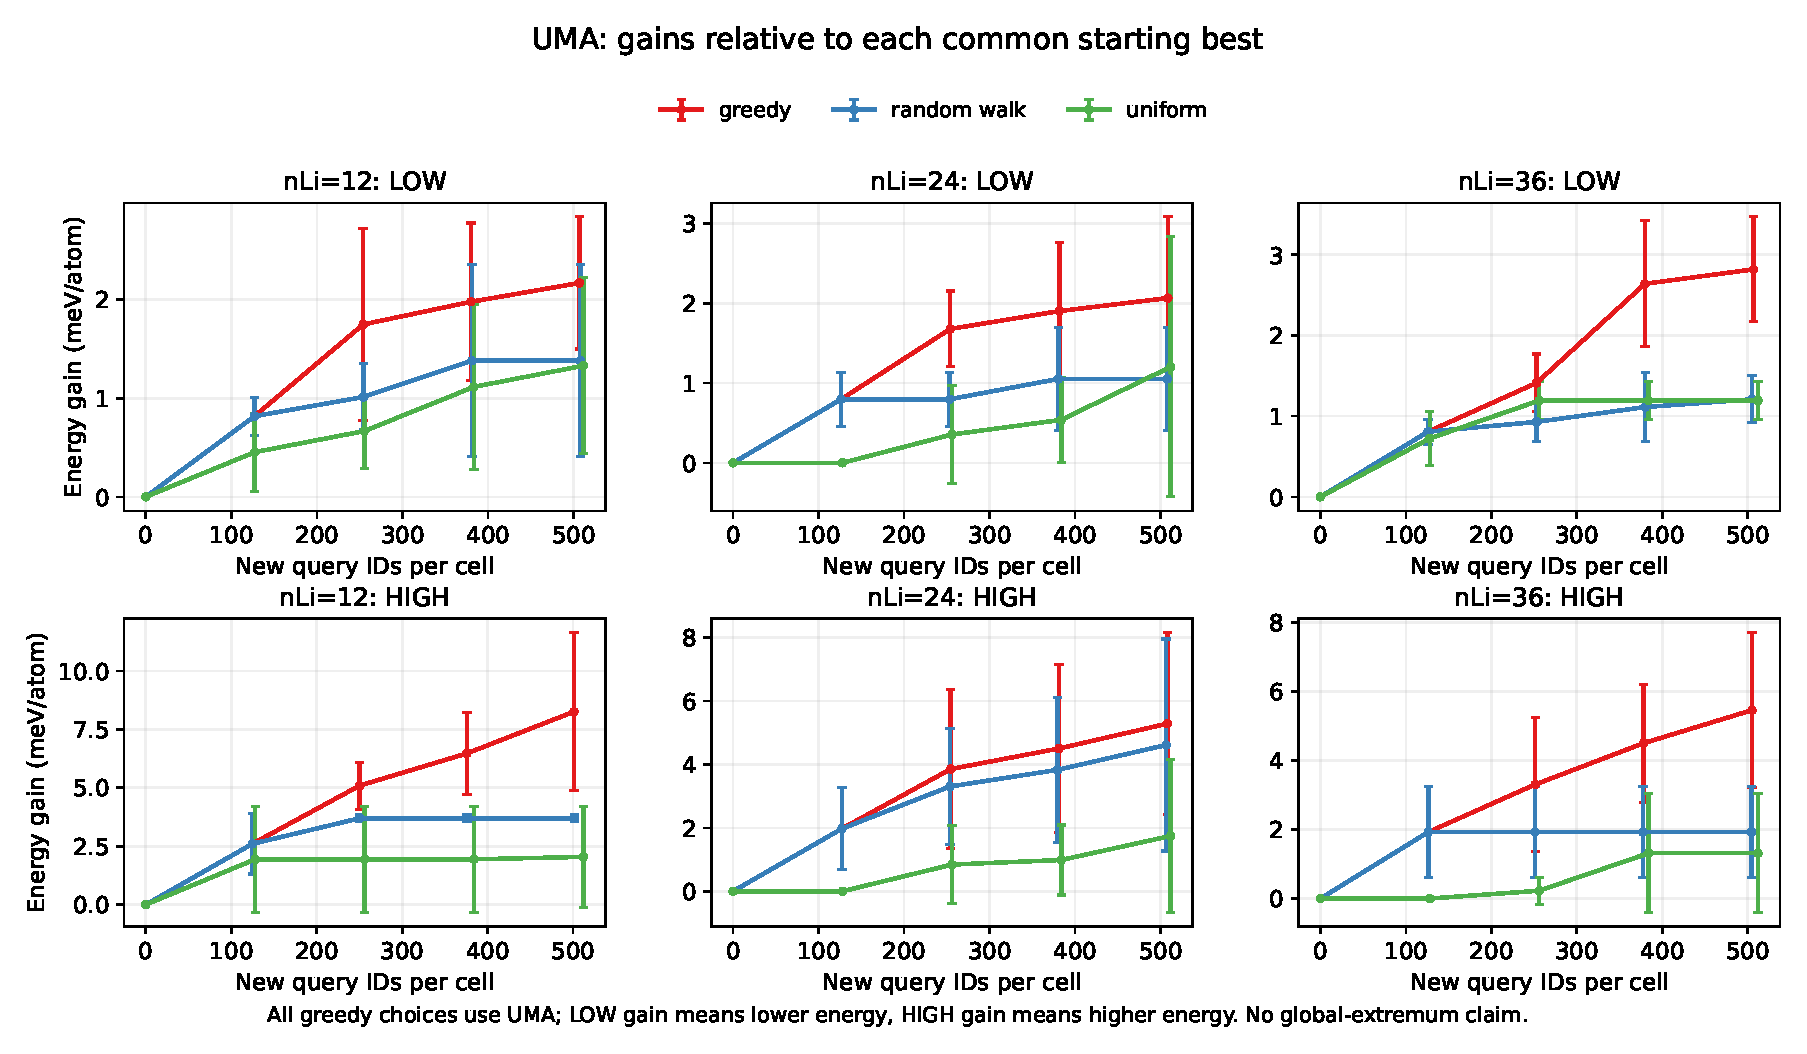
\includegraphics[width=\linewidth]{frontier_uma_best_gain.pdf}
\caption{Observed endpoint gains versus actual newly scored cell-query IDs.
Greedy and blind walks have identical first-step queries and fixed one-swap,
eight-neighbor budgets. Uniform has equal caps but different proposal
semantics. Best-so-far includes every evaluated neighbor and is monotone
by construction. Selected current paths are logged separately and may leave
an earlier best; the retained best and current state are different objects.
Error bars show three-seed sample SD.}
\end{figure}

No neural edit model is trained in this pilot. It separates label
redistribution from explicit oracle-guided search and cannot be treated as
a matched-edit comparison with the CVAE decoder. The new evaluations cover
49,570 geometry--teacher pairs, plus 574 separate rescoring evaluations of
287 distinct TRAIN seed masks. The pilot completes in 30.88 minutes within
its declared cap, with all raw checks passing.

Exact orbit filtering applies to all arms. Current-state uniqueness is
partly imposed by that filter, so it is not evidence of unrestricted
diversity. The saved diversity diagnostic instead uses the minimum Hamming
distance over parent symmetries, divided by two: the number of Li/vacancy
swaps separating two masks. The comparison uses the 16 current walk states
or the first 16 eligible uniform proposals without energy selection.
All coordinates remain unrelaxed. The results concern observed surrogate
endpoints, not global extrema, configurational entropy, equilibrium phase
stability, or DFT validation.



\section{Entropy: an exactly enumerable small-lattice test}
\subsection{Why uniqueness and thermodynamic counting differ}
The entropy pilot uses a new idealized O3 parent with 12 lithium sites,
derived from the N48 parent by crystallographic standardization and a
$2\times2\times1$ repeat of its conventional cell. It is not a Hu-archive
DFT geometry. Its 4,096 labelled masks form 87 symmetry orbits under 144
retained operations. All 87 representatives and 36 additional as-written
symmetry checks were evaluated by each MLIP. At half occupancy there are
$\binom{12}{6}=924$ labelled masks but only 17 orbits.

For novelty, each orbit is one pattern. For configurational entropy, its
multiplicity $g_o$ counts how many labelled-site microstates it represents.
Within fixed composition, and assuming equal energies within an orbit,
\begin{equation}
Z_{\rm rel}=\sum_o g_o e^{-\epsilon_o/(\kb T)},\qquad
\frac{S}{\kb}=\log Z_{\rm rel}+\frac{\langle\epsilon\rangle}{\kb T},
\label{eq:entropy}
\end{equation}
where $\epsilon_o=E_o-E_{\min}$ is the total cell energy relative to the
minimum of that composition, in eV; $\kb=8.617333262\times10^{-5}$\,eV/K;
and $T$ is temperature in K. $Z_{\rm rel}$ is the shifted partition sum;
a constant energy offset cancels exactly from entropy and heat capacity.
Using eV per atom instead would change the temperature scale incorrectly.
At infinite temperature all labelled masks have equal weight, giving
$S/\kb=\log\binom{12}{n}$, not the logarithm of the orbit count. A finite-cell
ground-state degeneracy also does not prove a bulk residual entropy.

The complete lattice gives an exact discrete sum for each set of
representative MLIP energies. It excludes vibrations, spin/electronic
degeneracy, strain, phase changes, and exchange of lithium between
compositions. It therefore tests an estimator, not experimental LCO entropy.
Numerical symmetry checks qualify the equal-energy assumption: over the 36
tested pairs, the maximum difference was 1.7961\,meV/cell for UMA and
0.03052\,meV/cell for MACE. At 100\,K these are 0.2084 and 0.00354 times
$\kb T$, respectively. At 100\,K this scale could appreciably affect
individual Boltzmann weights; its effect on entropy was not quantified.
Untested orientations are not bounded by the measured maximum.

\subsection{A learned proposal is not a Boltzmann distribution}
Three composition-only AR models are trained for 4,000 updates on a frozen
split of 57 TRAIN, 15 VAL, and 15 TEST orbits, with multiplicity weights and symmetry
augmentation. TEST energies are NaN in the learning export. Counts $n=3,6,9$
provide the estimator comparisons. The exact AR probability of every labelled
mask can be calculated as a product of its sequential probabilities; summing
them over the complete fixed-count space verifies normalization.

To guarantee full support, the actual proposal is
$q(x)=0.9q_{\rm AR}(x)+0.1/\binom{12}{n}$. For this enumerable pilot, independent
draws are sampled from the tabulated exact mixture; the ancestral AR sampler
is checked separately against its exact probabilities. Repeated masks are
retained and every draw counts toward the budget. Novelty rejection or
deduplication, as used in the N48 acquisition experiment, would change the
proposal law and invalidate these weights unless explicitly accounted for.
For $M$ draws, define
\begin{equation}
w_m=\frac{e^{-\epsilon(x_m)/(\kb T)}}{q(x_m)},\quad
\widehat Z_{\rm rel}=\frac1M\sum_m w_m,\quad
\widehat{\langle\epsilon\rangle}=\frac{\sum_mw_m\epsilon(x_m)}{\sum_m w_m}.
\end{equation}
No orbit multiplicity appears in these weights because the sampled objects
are labelled masks; an orbit-level proposal would need multiplicity factors.
The partition-sum sample mean is unbiased when the proposal covers all
states. The self-normalized energy estimate and entropy obtained by
substituting these estimates into Eq.~\ref{eq:entropy} have finite-sample
bias \cite{owen}. Weight effective sample size
$(\sum_m w_m)^2/\sum_m w_m^2$ describes concentration of importance weights,
not the number of independent Markov-chain samples. Uncorrected generated
frequencies estimate the generator's distribution, not a thermal distribution.
For a CVAE, the required proposal is the latent-marginal probability
$q(x)=\int p_\theta(x\mid z,c)p(z)\,dz$; a decoder likelihood at one sampled
$z$ cannot simply replace it. This pilot makes no CVAE entropy claim.
All estimator draws reuse the already tabulated MLIP energies. Their draw
budgets measure Monte Carlo error rather than additional static evaluations
or end-to-end GPU cost; enumeration is used here to validate the estimator.

\subsection{Density-of-states sampling and a necessary negative control}
Wang--Landau sampling estimates the density of states by flattening visits to
energy bins while refining the density estimate \cite{wanglandau}. We allow
up to 200,000 proposed swaps for each of three seeds, counts 3/6/9, two teachers,
and 16/32 bins: 36 bounded runs. All stopped after 14,000--40,000 swaps,
with 774,000 swaps in total. This deliberately small test supplies exact
nonempty-bin support, allowing two errors to be separated: replacing discrete
energies by bin midpoints, and estimating the number of microstates in each
bin. Flatness is checked every 1,000 swaps using $\min H\geq0.8\,\mathrm{mean}(H)$
over known occupied bins. Initially $\log f=1$; it halves after each flat
phase and stops below $10^{-4}$. This schedule is a project-specific
diagnostic, not proof of full-space coverage or bin-width convergence.

\begin{figure}[htbp]
\centering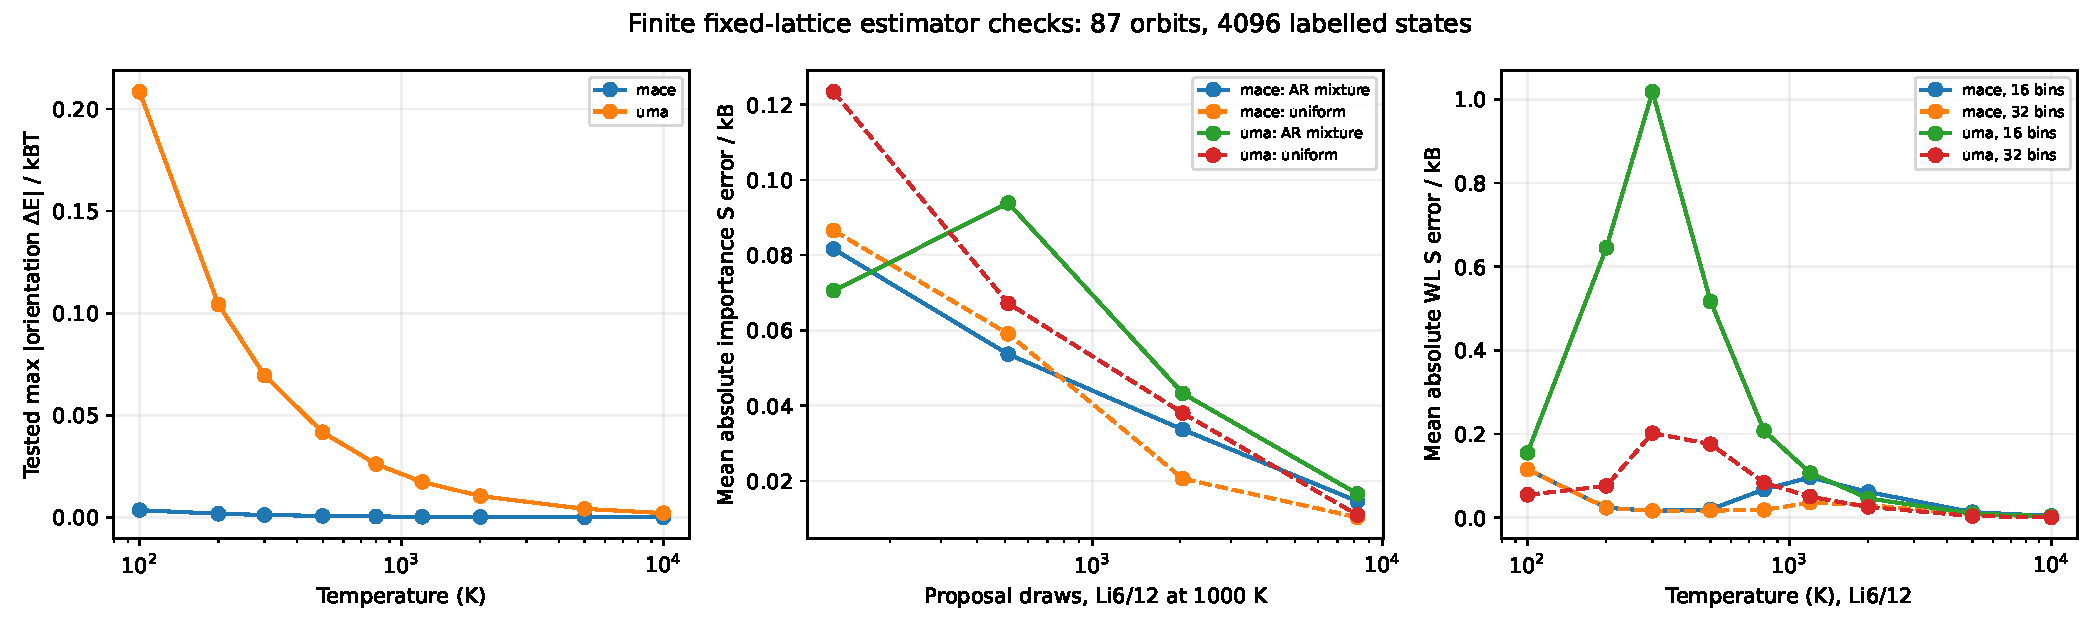
\includegraphics[width=\linewidth]{entropy_review.pdf}
\caption{Complete-lattice entropy controls. The energy differences in the
left panel are numerical symmetry checks; the middle panel compares
importance-corrected errors at equal sample budgets; the right panel
compares combined Wang--Landau entropy errors for 16/32 bins. The table below
separates midpoint binning from density-of-states estimation. These are
finite-cell MLIP calculations.}
\end{figure}

Ignoring orbit multiplicities gives a large error. For Li6/12 at 300\,K,
the correct representative-energy sum gives $S/\kb=3.26849$ for UMA and
5.35464 for MACE. Weighting each orbit equally instead gives 0.21254 and
1.75616. At infinite temperature the correct value is $\log924=6.82871$,
whereas equal orbit counting tends to $\log17=2.83321$. An independent
expansion over all 4,096 labelled masks reproduces the orbit-based entropy
within $2.66\times10^{-15}\kb$. This checks the combinatorics and formula,
not the physical accuracy of either teacher.

The largest AR probability-normalization discrepancy over exhaustive
fixed-count enumeration is $1.73\times10^{-7}$. Decoder samples are also
checked against the calculated proposal probabilities. At Li6/12, 1,000\,K,
and 8,192 draws, the following are mean absolute errors over draw seeds,
averaged within each fit and then over three independent terminal fits.
The uniform comparator has one proposal distribution and three draw seeds;
it does not have three different fitted models.

\begin{table}[htbp]
\centering
\caption{Learned importance proposal versus uniform labelled-mask sampling.
Entropy errors are in $\kb$ per periodic cell. The learned proposal contains
10\% uniform probability.}
\begin{tabular}{llrrr}\toprule
Teacher & Proposal & Entropy MAE & Naive MAE & Weight ESS/$M$\\\midrule
UMA & AR mixture & 0.01657 & 1.2916 & 0.1454\\
UMA & Uniform & 0.01096 & 1.3155 & 0.1795\\
MACE & AR mixture & 0.01460 & 1.0223 & 0.2352\\
MACE & Uniform & 0.01033 & 1.0462 & 0.2703\\\bottomrule
\end{tabular}
\end{table}

Importance correction is essential, but the learned proposal does not
outperform uniform sampling in this comparison. The composition-only model
was not trained to match a Boltzmann distribution at a specified temperature.
A useful next proposal would target weight concentration explicitly rather
than assume that a diverse or low-energy generator is automatically an
efficient partition-function sampler. Validation-selected checkpoint
sensitivities and all temperatures/counts/budgets remain in the full CSVs;
they are not substituted for the terminal primary comparison.

All 36 Wang--Landau runs met the frozen flatness/modification-factor
schedule. Nevertheless, at Li6/12 and 300\,K, doubling the bin count gives
the following distinct quantities:
\begin{table}[htbp]
\centering
\caption{Binning and sampling are separate approximations. ``Binned exact''
uses exact microstate counts with bin-midpoint energies. WL uses estimated
counts with the same midpoints. $\pm$ is the sample SD over three WL seeds.}
\begin{tabular}{llrrr}\toprule
Teacher & Bins & Discrete exact $S/\kb$ & Binned exact & WL mean $\pm$ SD\\\midrule
UMA & 16 & 3.26849 & 4.34857 & $4.28673\pm0.06677$\\
UMA & 32 & 3.26849 & 3.51230 & $3.47065\pm0.02877$\\
MACE & 16 & 5.35464 & 5.37712 & $5.34294\pm0.02633$\\
MACE & 32 & 5.35464 & 5.37592 & $5.34162\pm0.02637$\\\bottomrule
\end{tabular}
\end{table}
UMA's midpoint-only error is $+1.08008\kb$ with 16 bins and
$+0.24382\kb$ with 32 bins. This has not established quantitative bin-width
convergence at 300\,K, even though the sampling schedule completed. A small
total error can also result from cancellation between midpoint and
density-estimation errors. The two MLIPs' different exact entropies further
show that a numerically accurate estimator does not remove teacher
uncertainty.

\subsection{A proposal trained for the thermodynamic target}
The negative composition-only result suggests an objective mismatch:
reproducing a broad configuration distribution is not the same task as
placing probability where a thermal partition sum receives most of its
weight. A bounded follow-up therefore changes only within-composition TRAIN
weights to
\begin{equation}
w_o=A_n g_o\exp\!\left[-\frac{E_o-E_{\min,\mathrm{TRAIN},n}}
                              {\kb(1000\,\mathrm K)}\right],
\end{equation}
where $A_n$ preserves that composition's original total TRAIN multiplicity
weight. Energies are total eV per cell. VAL/TEST weights remain unchanged
and TEST energies remain NaN in the learning export. Perturbing held-out
energies leaves the training-row weights unchanged. The full reference was already
analyzed, so this is a theory-motivated development follow-up rather than a
fresh blind TEST.

Six new AR fits use the same three seeds, architecture, augmentation,
4,000-update budget, and terminal-checkpoint rule: three weighted using UMA
TRAIN energies and three using MACE TRAIN energies. Both teachers evaluate
every proposal distribution. All proposals retain the 10\% uniform mixture
and identical estimator budgets/draw seeds. All 216 uniform-control rows
reproduce the original baseline exactly; probability normalization differs
from one by at most $1.05\times10^{-7}$. The new weights are concentrated:
TRAIN orbit-weight ESS is approximately 1.2--4.2 for the three measured
compositions, a memorization risk rather than an acceptance criterion.

\begin{table}[htbp]
\centering\small
\caption{Temperature transfer of the 1,000 K-trained proposal. Entries are descriptive equal-composition averages over $n=3,6,9$ at 8,192 draws; MAE is in $k_{\rm B}$ per cell and ESS/$M$ is dimensionless. They are not averages of a physical entropy across compositions.}
\begin{tabular}{llrrrrr}\toprule
Teacher & $T$ (K) & AR MAE & Weighted MAE & Uniform MAE & W. ESS/$M$ & U. ESS/$M$\\\midrule
UMA & 300 & 0.026879 & 0.008345 & 0.020461 & 0.3038 & 0.1044\\
UMA & 1000 & 0.013095 & 0.004204 & 0.009409 & 0.7296 & 0.2495\\
UMA & 5000 & 0.001973 & 0.008512 & 0.001763 & 0.6274 & 0.8259\\
MACE & 300 & 0.020480 & 0.005252 & 0.016783 & 0.6374 & 0.2549\\
MACE & 1000 & 0.013710 & 0.003133 & 0.011170 & 0.7420 & 0.3006\\
MACE & 5000 & 0.001984 & 0.009692 & 0.001704 & 0.6515 & 0.8267\\
\bottomrule\end{tabular}
\end{table}


At the intended 1,000\,K target, own-teacher weighting improves entropy MAE
and weight ESS at every measured composition. The equal-composition MAE
falls from 0.013095 to 0.004204\,$\kb$/cell for UMA and from 0.013710 to
0.003133 for MACE; uniform gives 0.009409 and 0.011170. For Li6/12 alone,
the weighted MAEs are $0.005350\pm0.001264$ and
$0.004567\pm0.001314$, with SD across three fit means. The original
composition-only baseline is preserved rather than replaced by this result.

The gain is not universal. At 5,000\,K the 1,000\,K-trained proposal is too
concentrated: its MAEs are 0.008512/0.009692 for UMA/MACE, versus uniform
0.001763/0.001704. At 300\,K the descriptive equal-composition averages
improve both metrics, although individual cells can differ. Matching a
proposal to one thermodynamic target is therefore useful, while temperature
transfer still requires testing. Cross-teacher differences are retained in
the full table; three fits do not establish which training teacher is
generally superior.

\begin{figure}[htbp]
\centering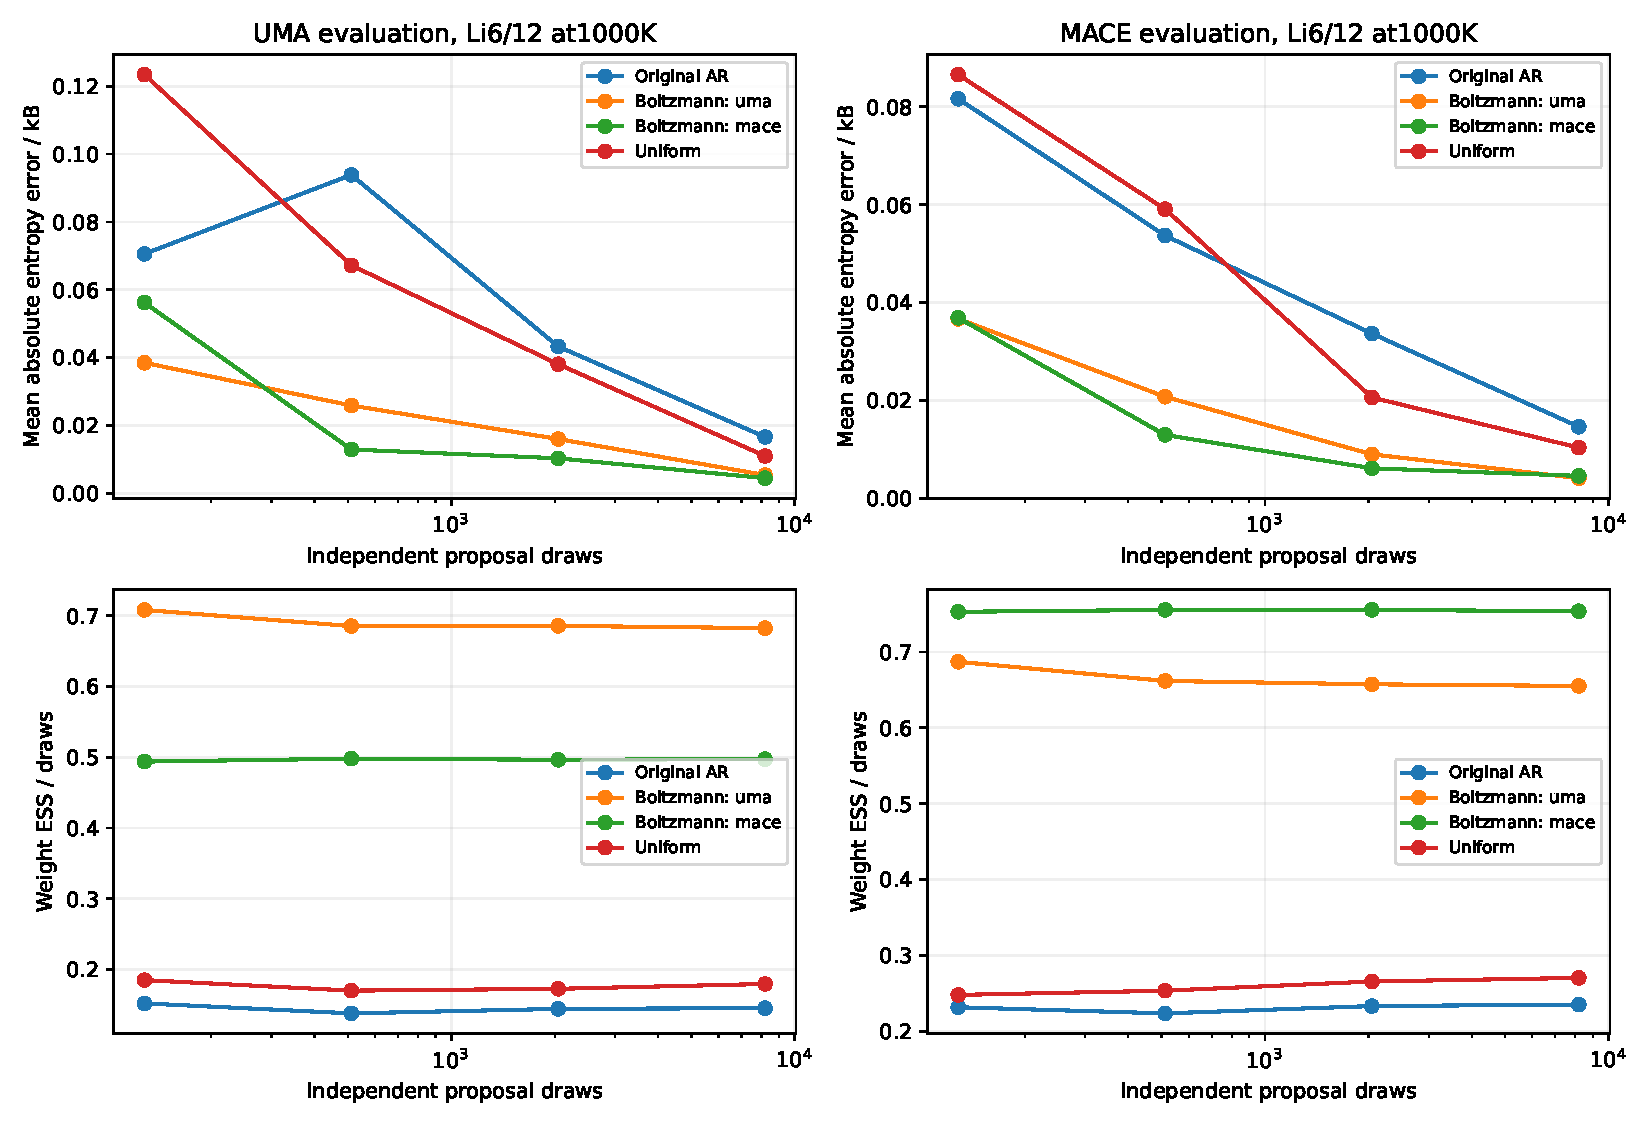
\includegraphics[width=\linewidth]{boltzmann_target_followup.pdf}
\caption{Li6/12 at 1,000 K: entropy MAE and weight ESS versus draw budget for
both teachers. The fixed-temperature training objective changes importance
efficiency without changing the reference. All sampled duplicates are retained.
Temperature transfer, including the negative 5,000 K result, is in the table.}
\end{figure}

A perfect Boltzmann proposal would make partition-sum importance weights
constant, minimizing their variance. That fact does not by itself minimize
finite-budget entropy error, which also contains the self-normalized energy
mean. We therefore evaluate entropy error and weight ESS separately. None of
these results turns the energy-bin-enriched N48 dataset into a density of
states: its adaptive selection law and novelty filtering differ from the
labelled-mask importance proposal used here.



\section{Scientific interpretation and reproducibility}
The autoregressive model remains the reference generator for subsequent
work. It is stochastic, respects composition exactly, and performs well
against the declared uniform and mutation controls in the broad three-bin
assessment. A CVAE should earn its additional latent machinery through a
matched improvement in sampling or reproducible control of an observed
property. The present dimension, KL-schedule, and auxiliary-head experiments
do not establish that improvement. They also do not show that the encoder
means are uninformative: the conditional probes and random-encoder controls
separate recoverable graph features from information that survives posterior
noise and guides prior generation.

The adaptive experiment should retain two distinct objectives: fidelity to
a fixed energy request and extension of the observed energy range. Updating
the upper endpoint can broaden what a range-defined LOW request means, so
these objectives can move in opposite directions. The same-row follow-up
shows that relabeling H0 and recomputing class weights already explains a
substantial balanced-yield gain, largely through HIGH requests. The
matched-edge comparisons do not show a consistent benefit from adding rows
for both model families. These are policy effects under the implemented
training procedure: class balancing and minibatches also change, and an H0
control using R1 edges still obtains information from acquired labels through
those edges. Further iteration should therefore be judged against its
same-lineage continuation using declared per-cell metrics, rather than by
training loss or a growing archive alone.

The entropy results answer a separate question. A temperature-specific
training measure produces a more useful importance proposal at 1,000\,K,
while its loss against uniform sampling at 5,000\,K makes the target
dependence explicit. This does not make the adaptively selected N48 archive
a density of states: its novelty rejection and acquisition probabilities
require separate treatment. The complete N12 lattice supplies a numerical
reference for estimator checks, including binning bias, not a physical
thermodynamic validation.

The next contributions can use the existing data and frozen results:
\begin{itemize}[leftmargin=*,itemsep=4pt]
\item \textbf{Ricardo: chemistry and teacher interpretation.}
Review representative configurations at both energy endpoints and where
UMA and MACE disagree. Check parent geometry, composition, energy units,
and symmetry conventions, and distinguish a valid vacancy mask from a
physically stable structure. Define a small, consistent later validation
set that separates fixed-geometry DFT checks from relaxation and phase
stability checks.
\item \textbf{Beihao: model and latent training.}
Reproduce the AR and $D=2$ references with their recorded budgets and
roles. Use the conditional probes, random-encoder controls, and sampled
posterior diagnostics to formulate one controlled change aimed at useful
sampled-latent information. Retain condition-only and shuffled controls,
and require an actual generated-property response rather than improvement
of the auxiliary predictor alone. Deliver the checkpoint, run receipt,
and per-condition learning and control diagnostics.
\item \textbf{Varad: evaluation and statistics.}
Regenerate the paired tables and figures from the bound CSVs, retaining
all attempted proposals in the appropriate denominators. Audit fixed
versus moving thresholds, novelty histories, paired seed differences,
and the distinction between SD and confidence intervals. Keep entropy
weight ESS separate from independence and accuracy, and report binning
error separately from density estimation. Deliver a reproducible analysis
with per-cell results, source checks, and cost receipts.
\end{itemize}

Physical validation remains a separate stage. Independent DFT labels under
consistent settings, geometry relaxation, possible departures from O3,
cell-size effects, and finite-temperature stability must be assessed before
claiming improved MLIP training data or predictive recycling simulations.
The present run supplies neither a validated relaxed-coordinate generator
nor evidence that an MLIP fine-tuned on its proposals would remain stable
in dynamics. Those claims require their own comparisons and observables.


\paragraph{Data-boundary and execution record.}
All proposed attempts, raw worker outputs, frozen task files, input/source
hashes, and informative failures remain in the run archive. A first MACE
startup used an incompatible UMA environment and failed before claiming a
MACE scoring task; the retry used the dedicated MACE interpreter and the same
model/input. An initial identity-boundary preparation was too broad and was
replaced before any energy evaluation; its unscored attempts were retained
as known history. The correction preserves inherited H0 TRAIN identities
instead of newly declaring them protected. The subsequent phase-two latent
identity boundary is added before later acquisition, with a documented
driver handoff rather than a silent change to frozen source. Historical
assessment exposure and inherited TRAIN/protected overlaps are disclosed
in the existing boundary receipts; this study is development evidence, not
a newly blind TEST claim.

The code uses one assigned GPU per worker, exact model heads/checkpoints,
FP32 neural fitting/MLIP inference, and disabled TF32 shortcuts. Entropy sums
and importance calculations use float64. Model fitting, scoring, and
substantial analysis run within existing compute allocations. Raw results are
preserved; compact report assets and receipts make the conclusions reviewable
without copying all checkpoints or protected identities into the report.
The campaign completes 166 generative fits (520,000 optimizer updates) and
469,672 geometry--teacher static evaluations, including repeat evaluations
required by separately frozen comparisons. This is an evaluation-event count,
not the number of globally unique physical geometries. The final allocation
receipt reports all four Slurm allocations, including startup, idle time and
failed technical subprocesses, with GPU-node-hours defined as allocated
GPU-device hours divided by four. Shared-node allocations can overlap on the
same physical node. This estimate is distinct from an official posted charge;
the compact packet's \texttt{resource\_receipt.json} records final
usage of 28.8799 GPU-node-hours (115.5194 allocated
GPU-device hours), below the 150 GPU-node-hour limit. All four allocations
have ended; three idle allocations were explicitly released and the final
shared workers exited normally.


\begin{thebibliography}{9}
\bibitem{uma} B. M. Wood et al.
UMA: A Family of Universal Models for Atoms (2025).
\url{https://arxiv.org/abs/2506.23971}.
\bibitem{macefoundation} MACE developers.
Foundation models: MACE-MH-1/0. Official model documentation,
accessed November 13, 2026.
\url{https://mace-docs.readthedocs.io/en/latest/guide/foundation_models.html}.
\bibitem{wakamiya} T. Wakamiya and A. Ishikawa.
Artificial catalyst generation for the oxygen reduction reaction using
conditional variational autoencoder and atomistic calculations.
\emph{npj Computational Materials} 12, 206 (2026).
\url{https://doi.org/10.1038/s41524-026-02075-0}.
\bibitem{kingma} D. P. Kingma and M. Welling.
Auto-Encoding Variational Bayes. ICLR (2014).
\url{https://arxiv.org/abs/1312.6114}.
\bibitem{fu} H. Fu et al.
Cyclical Annealing Schedule: A Simple Approach to Mitigating KL Vanishing.
NAACL-HLT, 240--250 (2019).
\url{https://doi.org/10.18653/v1/N19-1021}.
\bibitem{wanglandau} F. Wang and D. P. Landau.
Efficient, Multiple-Range Random Walk Algorithm to Calculate the Density of
States. \emph{Physical Review Letters} 86, 2050--2053 (2001).
\url{https://doi.org/10.1103/PhysRevLett.86.2050}.
\bibitem{owen} A. B. Owen.
\emph{Monte Carlo theory, methods and examples}, Chapter 9,
Sections 9.1--9.3 (2013).
\url{https://artowen.su.domains/mc/Ch-var-is.pdf}.
\end{thebibliography}

\end{document}
